\documentclass[]{kclthesis}

\modulecode{7CCSMPRJ} 
\submissiontitle{Individual Project Submission 2024-2025}
\studentnumber{K24087939}
\programme{Computational Finance M.Sc.}
\supervisor{Riaz Ahmad}
\wordcount{14665
}
\title{Explainable Deep Learning for Portfolio Optimisation}
\author{Ingrid Pérez Aguilera}
\ReleaseProject{1} 
\department{Informatics} 

\usepackage{float}
\usepackage{hyperref}
\usepackage[utf8]{inputenc}
\usepackage{graphbox}
\usepackage{pgfgantt}
\usepackage{nomencl}
\usepackage[acronym]{glossaries}
\usepackage{amsmath}
\usepackage{algorithm}
\usepackage{algpseudocode}
\usepackage{bm}

\newtheorem{theorem}{Theorem}[section]
\newtheorem{exa}{Example}[section]
\newtheorem{corollary}[theorem]{Corollary}
\newtheorem{lemma}[theorem]{Lemma}
\newtheorem{proposition}[theorem]{Proposition}

\theoremstyle{definition}
\newtheorem{definition}[theorem]{Definition}
\newtheorem{remark}[theorem]{Remark}
\newtheorem{notation}[theorem]{Notation}
\newtheorem{assumption}[theorem]{Assumption}
\newtheorem{conjecture}[theorem]{Conjecture}

\newcommand{\ind}{1\hspace{-2.1mm}{1}} %Indicator Function
\newcommand{\I}{\mathtt{i}}
\newcommand{\D}{\mathrm{d}}
\newcommand{\E}{\mathrm{e}}
\newcommand{\RR}{\mathbb{R}}
\newcommand{\sgn}{\mathrm{sgn}}
\newcommand{\atanh}{\mathrm{arctanh}}
\def\blue#1{\textcolor{blue}{#1}}
\def\red#1{\textcolor{red}{#1}}

\setcounter{secnumdepth}{5}
\setlength{\marginparwidth}{2cm} % Adjust marginparwidth to avoid todonotes issues
\renewcommand{\contentsname}{Table of Contents}

\makeglossaries
\makenomenclature
\begin{document}
\pagenumbering{gobble}

%%%%% Cover page
\maketitle 

%%%%% Empty page
\newpage
\thispagestyle{empty}
\mbox{}
\newpage

%%%%% Abstract and acknowledgements
\chapter*{Abstract}
	It is a précis of the report (normally in one page), which should include:
\begin{itemize}
	\item A brief introduction to the project objectives
	\item A brief description of the main work of the project
	\item A brief description of the contributions, major findings, results achieved and principal conclusion of the project
\end{itemize}

\chapter*{Acknowledgements} 

I would like to express my gratitude to my supervisor, Dr. Riaz Ahmad, for his guidance and support throughout this project. I would also like to thank my Master's colleagues for being there during this journey and the valuable discussions we had.

I would like to convey my appreciation to my partner for his unwavering support, encouragement and all the help in reviewing the code and the report. I would also like to acknowledge my family's continuous support and encouragement throughout my studies.

%%%%% Table of contents
\pagenumbering{roman}
\setcounter{tocdepth}{2}
\doublespacing
\tableofcontents
\newpage

%%%%% List of figures
\listoffigures
\newpage

%%%%% List of tables
\listoftables
\newpage

%%%%% List of algorithms
\listofalgorithms
\newpage

%%%%% Nomenclature
% All abbreviations and symbols used in the report must be listed and defined in alphabetic order.
\nomenclature{\(c\)}{Speed of light in a vacuum}
\nomenclature{\(h\)}{Planck constant}
\printnomenclature
\newpage

%%%%% List of acronyms
\newglossaryentry{financialmarkets}
{
    name=Financial Markets,
    text={financial markets},
    description={Marketplaces where people trade financial securities, commodities, and other fungible items of value at low transaction costs and at prices that reflect supply and demand}
}
\newglossaryentry{algorithmictrading}
{
    name=Algorithmic Trading,
    text={algorithmic trading},
    description={Use of computer algorithms to automate trading decisions and execute trades in financial markets}
}
\newglossaryentry{machinelearning}
{
    name=Machine Learning,
    description={Subset of artificial intelligence that enables systems to learn from data and improve their performance over time without being explicitly programmed}
}
\newglossaryentry{deeplearning}
{
    name=Deep Learning,
    description={Subset of machine learning that uses neural networks with many layers to learn from large amounts of data, enabling the model to automatically learn complex patterns and representations}
}
\newglossaryentry{reinforcementlearning}
{
    name=Reinforcement Learning,
    description={Subset of machine learning where an agent learns to make decisions by taking actions in an environment to maximise cumulative reward}
}
\newglossaryentry{deepreinforcementlearning}
{
    name=Deep Reinforcement Learning,
    description={Combination of deep learning and reinforcement learning, where deep neural networks are used to approximate the value function or policy in reinforcement learning tasks}
}
\newglossaryentry{artificialintelligence}
{
    name=Artificial Intelligence,
    description={Simulation of human intelligence processes by machines enabling them to perform tasks that typically require human intelligence, such as visual perception, speech recognition, decision-making, and language translation}
}
\newglossaryentry{explainableai}
{
    name=Explainable Artificial Intelligence,
    description={Methods and techniques in the application of artificial intelligence that make the results of the models understandable by humans, providing insights into how decisions are made}
}
\newglossaryentry{portfoliooptimisation}
{
    name=Portfolio Optimisation,
    text={portfolio optimisation},
    description={Process of selecting the best distribution of assets in a portfolio to achieve specific investment goals, such as maximising returns or minimising risk, while considering constraints and preferences}
}
\newglossaryentry{advantageactorcritic}
{
    name=Advantage Actor-Critic,
    description={Algorithm that uses both an actor (policy) and a critic (value function) to learn optimal policies by estimating the advantage of actions taken}
}
\newglossaryentry{proximalpolicyoptimisation}
{
    name=Proximal Policy Optimisation,
    description={Algorithm that optimises policies by ensuring that updates to the policy are not too large, maintaining a balance between exploration and exploitation}
}
\newglossaryentry{deepdeterministicpolicygradient}
{
    name=Deep Deterministic Policy Gradient,
    description={Algorithm that uses deep neural networks to learn policies for continuous action spaces, combining the benefits of deep learning and policy gradient methods}
}
\newglossaryentry{twindelayeddeepdeterministicpolicygradient}
{
    name=Twin Delayed Deep Deterministic Policy Gradient,
    description={Extension of \Gls{deepdeterministicpolicygradient} that addresses the overestimation bias in value function estimation by using two critic networks and delaying policy updates}
}
\newglossaryentry{softactorcritic}
{
    name=Soft Actor-Critic,
    description={Algorithm that combines the benefits of off-policy learning and entropy regularisation, allowing for more exploration and better stability in learning policies for continuous action spaces}
}
\newglossaryentry{shapleyadditiveexplanations}
{
    name=SHapley Additive exPlanations,
    description={Method for interpreting machine learning models by assigning each feature an importance value for a particular prediction, based on cooperative game theory}
}
\newglossaryentry{localinterpretablemodelagnosticexplanations}
{
    name=Local Interpretable Model-agnostic Explanations,
    description={Technique for explaining the predictions of any machine learning model by approximating it with a locally interpretable model, allowing users to understand the model's behaviour in a specific instance}
}
\newglossaryentry{featureimportance}{
    name=Feature Importance,
    description={Technique for determining the contribution of each feature in a machine learning model to its predictions, helping to identify which features are most influential}
}
\newglossaryentry{rewardfunction}{
    name=Reward Function,
    text={reward function},
    description={Function that defines the feedback signal received by an agent in reinforcement learning, guiding the agent's learning process by providing rewards or penalties based on its actions}
}
\newglossaryentry{hyperparameters}{
    name=Hyper-parameter,
    text={hyper-parameter},
    description={Parameter that is set before the learning process begins and control the learning process of a machine learning model, such as learning rate, batch size, and number of layers in a neural network}
}
\newglossaryentry{efficientfrontier}{
    name=Efficient Frontier,
    text={efficient frontier},
    description={Set of optimal portfolios that offer the highest expected return for a given level of risk, or the lowest risk for a given level of expected return, in the context of portfolio optimisation}
}
\newglossaryentry{modernportfoliotheory}{
    name=Modern Portfolio Theory,
    text={Modern Portfolio Theory},
    description={Investment theory that aims to construct a portfolio of assets that maximises expected return for a given level of risk, or minimises risk for a given level of expected return, through diversification}
}
\newglossaryentry{supervisedlearning}{
    name=Supervised Learning,
    description={Machine learning task where a model is trained on labelled data to learn a mapping from inputs to outputs}
}
\newglossaryentry{unsupervisedlearning}{
    name=Unsupervised Learning,
    description={Machine learning task where a model learns patterns or structures in unlabelled data without explicit supervision}
}
\newglossaryentry{deepneuralnetwork}{
    name=Deep Neural Network,
    plural={deep neural networks},
    description={Type of artificial neural network with a succession of layers of non-linear transformations capable of learning a representation of the data with various levels of abstraction}
}
\newglossaryentry{markovdecisionprocess}{
    name=Markov Decision Process,
    text={Markov Decision Process},
    description={Mathematical model for sequential-decision making where the outcomes are uncertain, characterised by states, actions, rewards and a transition function}
}
\newglossaryentry{partiallyobservablemarkovdecisionprocess}{
    name=Partially Observable Markov Decision Process,
    text={Partially Observable Markov Decision Process},
    description={Extension of \Gls{markovdecisionprocess} where the agent does not have access to the complete state information, requiring the use of belief states or observations to make decisions}
}
\newglossaryentry{bellmanequations}{
    name=Bellman Equations,
    text={Bellman equations},
    description={Set of equations that describe the relationship between the value of a state or action and the values of subsequent states or actions in dynamic programming and reinforcement learning} 
}
\newglossaryentry{entropy}{
    name=Entropy,
    text={entropy},
    description={Measure of uncertainty or randomness in a system, often used in the context of information theory and reinforcement learning to encourage exploration}
}
\newglossaryentry{meanvarianceoptimisation}{
    name=Mean-Variance Optimisation,
    description={Investment strategy that aims to construct a portfolio of assets that maximises expected return for a given level of risk, or minimises risk for a given level of expected return}
}
\newglossaryentry{python}{
    name=Python,
    description={Interpreted, object-oriented, high-level programming language}
}
\newglossaryentry{blackbox}{
    name=Black Box,
    text={black box},
    plural=black boxes,
    description={Term used to describe a system or model whose internal workings are not transparent or easily understood}
}
\newglossaryentry{exploration}{
    name=Exploration,
    text={exploration},
    description={Process of investigating and experimenting with different actions or strategies to discover their effects and improve decision-making}
}
\newglossaryentry{exploitation}{
    name=Exploitation,
    text={exploitation},
    description={Process of leveraging known information to make decisions or take actions that are expected to yield the highest reward}
}

\newacronym{dl}{DL}{\Gls{deeplearning}}
\newacronym{ml}{ML}{\Gls{machinelearning}}
\newacronym{rl}{RL}{\Gls{reinforcementlearning}}
\newacronym{drl}{DRL}{\Gls{deepreinforcementlearning}}
\newacronym{a2c}{A2C}{\Gls{advantageactorcritic}}
\newacronym{ppo}{PPO}{\Gls{proximalpolicyoptimisation}}
\newacronym{ddpg}{DDPG}{\Gls{deepdeterministicpolicygradient}}
\newacronym{td3}{TD3}{\Gls{twindelayeddeepdeterministicpolicygradient}}
\newacronym{sac}{SAC}{\Gls{softactorcritic}}
\newacronym{shap}{SHAP}{\Gls{shapleyadditiveexplanations}}
\newacronym{lime}{LIME}{\Gls{localinterpretablemodelagnosticexplanations}}
\newacronym{ai}{AI}{\Gls{artificialintelligence}}
\newacronym{xai}{XAI}{\Gls{explainableai}}
\newacronym{mpt}{MPT}{\Gls{modernportfoliotheory}}
\newacronym{dnn}{DNN}{\Gls{deepneuralnetwork}}
\newacronym{mdp}{MDP}{\Gls{markovdecisionprocess}}
\newacronym{pomdp}{POMDP}{\Gls{partiallyobservablemarkovdecisionprocess}}
\newacronym{dqn}{DQN}{Deep Q-Network}
\newacronym{a3c}{A3C}{Asynchronous Advantage Actor-Critic}
\newacronym{trpo}{TRPO}{Trust Region Policy Optimisation}
\newacronym{dpg}{DPG}{Deterministic Policy Gradient}
\newacronym{sma}{SMA}{Simple Moving Average}
\newacronym{ema}{EMA}{Exponential Moving Average}
\newacronym{macd}{MACD}{Moving Average Convergence Divergence}
\newacronym{rsi}{RSI}{Relative Strength Index}
\newacronym{cci}{CCI}{Commodity Channel Index}
\newacronym{atr}{ATR}{Average True Range}
\newacronym{adx}{ADX}{Average Directional Index}
\newacronym{dx}{DX}{Directional Movement Index}
\newacronym{pdi}{PDI}{Positive Directional Index}
\newacronym{mdi}{MDI}{Negative Directional Index}
\newacronym{roc}{ROC}{Rate of Change}
\newacronym{vix}{VIX}{Volatility Index}
\newacronym{vftse}{VFTSE}{Volatility FTSE}
\newacronym{vstoxx}{VSTOXX}{Volatility Euro Stoxx}
\newacronym{vxd}{VXD}{Volatility DW30}
\newacronym{ftse100}{FTSE 100}{Financial Times Stock Exchange 100 Index}
\newacronym{sp500}{S\&P 500}{Standard and Poor's 500 Index}
\newacronym{dw30}{DW30}{Dow Jones 30 Index}
\newacronym{eurostoxx50}{Euro Stoxx 50}{Euro Stoxx 50 Index}
\newacronym{us}{U.S.}{United States}
\newacronym{dxy}{DXY}{\acrshort{us} Dollar Index}
\newacronym{exy}{EXY}{Euro Index}
\newacronym{bxy}{BXY}{British Pound Currency Index}
\newacronym{irx}{IRX}{3-Month Treasury Yield}
\newacronym{fvx}{FVX}{5-Year Treasury Yield}
\newacronym{tnx}{TNX}{10-Year Treasury Yield}
\newacronym{mvo}{MVO}{\Gls{meanvarianceoptimisation}}
\newacronym{lstm}{LSTM}{Long Short-Term Memory}
\newacronym{mape}{MAPE}{Mean Absolute Percentage Error}
\newacronym{pca}{PCA}{Principal Component Analysis}
\newacronym{djia}{DJIA}{Dow Jones Industrial Average}
\newacronym{eu}{EU}{European Union}
\newacronym{saac}{SAAC}{Synchronous Advantage Actor Critic}
\newacronym{usd}{USD}{United States Dollar}
\newacronym{eur}{EUR}{Euro}
\newacronym{gbp}{GBP}{British Pound}
\newacronym{jpy}{JPY}{Japanese Yen}
\newacronym{aud}{AUD}{Australian Dollar}
\newacronym{cad}{CAD}{Canadian Dollar}
\newacronym{cny}{CNY}{Chinese Yuan}
\newacronym{chf}{CHF}{Swiss Franc}
\newacronym{hkd}{HKD}{Hong Kong Dollar}
\newacronym{krw}{KRW}{South Korean Won}
\newacronym{inr}{INR}{Indian Rupee}
\newacronym{ohlcv}{OHLCV}{Open, High, Low, Close, Volume}
\newacronym{var}{VaR}{Value at Risk}
\newacronym{aiact}{AI Act}{Artificial Intelligence Act}
\newacronym{mifid}{MiFID II}{Markets in Financial Instruments Directive II}
\newacronym{uk}{UK}{United Kingdom}
\newacronym{fca}{FCA}{Financial Conduct Authority}
\newacronym{llm}{LLM}{Large Language Model}
\newacronym{ip}{IP}{Intellectual Property}
\newacronym{bcs}{BCS}{British Computer Society}
\newacronym{iet}{IET}{The Institution of Engineering and Technology}
\newacronym{mse}{MSE}{Mean Squared Error}
\printglossary
\printglossary[type=\acronymtype]
\newpage

%%%%% Main content
\pagenumbering{arabic}
\onehalfspacing
\setlength{\parindent}{0pt}
\setlength{\parskip}{6pt}


%%%%%% Chapters
\doublespacing

\chapter{Introduction}\label{ch:introduction}
\chapter{Background} \label{ch:background}

This chapter provides an overview of the problem of portfolio optimisation in the financial domain, followed by a comprehensive explanation of the fundamentals of \acrfull{dl} and \acrfull{rl}, including the relevant algorithms in the field of \acrfull{drl}. In addition, it discusses the need for explainability in \acrfull{ml} and the main techniques used to achieve it: \acrfull{shap}, \acrfull{lime} and \Gls{featureimportance}. Finally, it presents the state of the art in portfolio optimisation using \acrshort{drl} and the recent advancements in explainability techniques in the field. 

\section{Portfolio Optimisation} \label{sec:portfoliooptimisation}

\Gls{portfoliooptimisation} is the process of selecting optimal weights for a portfolio of assets in order to maximise expected returns for a given level of risk, or conversely, to minimise risk for a given level of expected returns \cite{Sato2019}. In mathematical terms, the problem requires finding a solution to the specified objective function, which is typically a function of the expected returns and the risk associated with the portfolio \cite{Bruce2014}. The task becomes further complicated if a time dimension is introduced, as the portfolio weights need to be adjusted over time to capture the changes in market conditions and asset prices \cite{Li2019}. 

\subsection{Modern Portfolio Theory}

There exist several traditional frameworks that formalise the problem of portfolio allocation. Markowitz's \acrfull{mpt} was proposed in 1952 \cite{Markowitz1952} and it provides a mathematical framework where investors choose optimal portfolios based on risk and return, by either minimising the risk given a specified return or, maximising the return given a specified risk \cite{kent}. The theory extends the concept of diversification by suggesting that owning financial assets of different kinds is less risky than owning assets of the same kind, due to the correlations between assets. 

The main assumptions in \acrshort{mpt} are:
\begin{itemize}
    \item investors are risk-averse, rational, and seek to maximise return for a given risk;
	\item returns are normally distributed;
	\item markets are frictionless, meaning there are no transaction costs; and
	\item assets are infinitely divisible.
\end{itemize}

Under these assumptions, portfolio risk and return can be modelled as an optimisation problem. Let $\mathbf{w} = \left(w_1, w_2, \dots, w_N\right)^T$ denote the portfolio weight vector, where each $w_i$ indicates the proportion of capital allocated to asset $i$, subject to the budget constraint:
\begin{equation}
    \sum_{i=1}^{N} w_i = 1 \quad \Leftrightarrow \quad \mathbf{w}^T \mathbf{1} = 1
\end{equation}
with $\mathbf{1} \in \mathbb{R}^N$ being a vector of ones, and subject to the non-negativity constraint, meaning that short-selling is not allowed:
\begin{equation}
    w_i \geq 0 \quad \forall i = 1, 2, \dots, N.
\end{equation}

Let $\boldsymbol{\mu} = \left(R_1, R_2, \dots, R_N\right)^T$ represent the vector of expected returns, and $\Sigma \in \mathbb{R}^{N \times N}$ the covariance matrix of asset returns. The expected return of the portfolio is then given by:
\begin{equation}
    R_p = \mathbf{w}^T \boldsymbol{\mu},
\end{equation}
and the portfolio risk is quantified by the variance of returns:
\begin{equation}
    \sigma_p^2 = \mathbf{w}^T \Sigma \mathbf{w}.
\end{equation}

This formulation provides the foundation for solving the mean-variance optimisation problem, by either:
\begin{itemize}
    \item minimising portfolio variance $\sigma_p^2$ subject to a target expected return $R_p$, or
    \item maximising expected return $R_p$ subject to a risk constraint $\sigma_p$.
\end{itemize}

The Markowitz mean-variance optimisation problem can be expressed as:
\begin{equation}
\begin{aligned}
    \min_{\mathbf{w}} \quad & \mathbf{w}^T \Sigma \mathbf{w} \\
    \text{subject to} \quad &
    \begin{cases}
        \mathbf{w}^T \boldsymbol{\mu} = R_p \\
        \mathbf{w}^T \mathbf{1} = 1 \\
        \mathbf{w} \geq 0
    \end{cases}
\end{aligned}
\end{equation}

Solving the mean-variance optimisation problem for varying levels of target return leads to a set of optimal portfolios that form the \gls{efficientfrontier}. It is typically visualised in a risk-return space, where the x-axis represents the risk (standard deviation) and the y-axis represents the expected return, as shown in Figure \ref{fig:efficient_frontier}. Portfolios below the curve are suboptimal, while those on the frontier represent the best achievable combinations of risk and return.

\begin{figure}[ht]
    \centering
    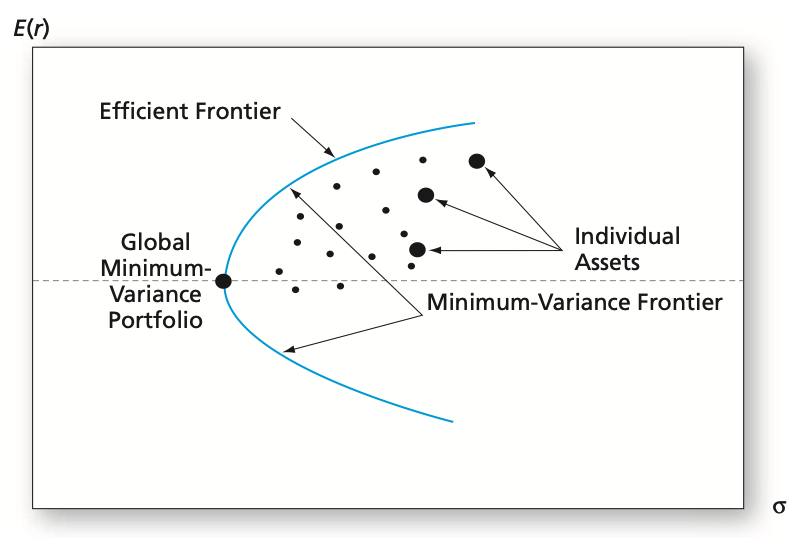
\includegraphics[width=0.8\textwidth]{figures/markowitz-efficient-frontier.png}
    \caption{Efficient Frontier in Risk-Return Space. \cite{Bodie2014}}
    \label{fig:efficient_frontier}
\end{figure}

Despite the simplicity in the formulation of \acrshort{mpt}, its assumptions do not reflect the behaviour of real markets. Moreover, modern markets are dynamic, non-stationary, and feature non-linear relationships, which have driven research into other approaches better suited to capture the complexities of modern financial markets. 
 
\section{Deep Reinforcement Learning} \label{sec:deepreinforcementlearning}

\acrlong{ml} is a branch of \acrfull{ai} that focuses on the use of data and algorithms to imitate the way humans learn, gradually improving their accuracy over time \cite{IBM2021}. There are three main tasks in \acrshort{ml} \cite{Francois-Lavet2018}:

\begin{itemize}
    \item \textbf{\Gls{supervisedlearning}}: Task of training a classification or regression model from labelled training data, where the model learns to map inputs to outputs based on examples.
    \item \textbf{\Gls{unsupervisedlearning}}: Task of drawing inferences from datasets consisting of unlabelled input data, where the model learns to identify patterns or structures in the data.
    \item \textbf{\acrlong{rl}}: Task of training an agent to sequentially make decisions by taking actions in an environment with the goal of maximising cumulative reward, using feedback from the environment to learn an optimal strategy.
\end{itemize}

\acrlong{dl} is a set of methods and techniques to solve such \acrshort{ml} tasks, specially in supervised and unsupervised learning tasks. \acrshort{dl} focuses on the use of \acrfull{dnn} \cite{Goodfellow2016}, which are characterised by a succession of layers of non-linear transformation that allow the model to learn a representation of the data with various levels of abstraction.

Therefore, \acrfull{drl} combines \acrfull{dl} and \acrfull{rl} to solve sequential decision-making problems with high-dimensionality in the environment representation. This approach has gained significant attention in recent years due to its success in various applications, including robotics \cite{Tang2024} and game playing \cite{Silver2016, Shao2019}.

\subsection{Reinforcement Learning} \label{sec:reinforcementlearning}

As mentioned, \acrshort{rl} is a type of \acrshort{ml} that solves the problem of sequential decision-making through continuous interaction with an environment. The agent learns to take actions given a representation of the environment's state with the goal of optimising a pre-defined notion of reward. The agent learns by successively adjusting its policy based on its observations and interactions with the environment. 

The \acrshort{rl} problem can be formalised as a discrete-time stochastic control process where an agent interacts with the environment. At each time step $t$, the agent observes the state of the environment $s_t \in \mathcal{S}$, takes an action $a_t \in \mathcal{A}$ to obtain a reward $r_t \in \mathbb{R}$ and transition to a new state $s_{t+1} \in \mathcal{S}$, where $\mathcal{S}$ is the state space and $\mathcal{A}$ is the action space \cite{Francois-Lavet2018}. The agent's interaction with the environment is visually represented in Figure \ref{fig:agent_environment_interaction}.

\begin{figure}[ht]
    \centering
    \begin{tikzpicture}[>=stealth]
    % Nodes
    \node[draw, rectangle, minimum width=2cm, minimum height=1cm] (agent) {Agent};
    \node[draw, rectangle, minimum width=2.8cm, minimum height=1cm, right=5cm of agent] (env) {Environment};

    % Coordinates for paths
    \coordinate (top1) at ($(env.north)+(0,1.5)$);
    \coordinate (top2) at ($(agent.north)+(0,1.5)$);

    \coordinate (bot1) at ($(env.south)+(0,-1.5)$);
    \coordinate (bot2) at ($(agent.south)+(0,-1.5)$);

    % Arrows
    \draw[->] (agent) -- node[above, midway] {Action $a_t$} (env);
    \draw[->] (env.north) -- (top1) -- node[above] {State $s_t$} (top2) -- (agent.north);
    \draw[->] (env.south) -- (bot1) -- node[below] {Reward $r_t$} (bot2) -- (agent.south);
\end{tikzpicture}
    \caption{Agent interaction with environment}
    \label{fig:agent_environment_interaction}
\end{figure}

A discrete time stochastic control process can be formalised as a \acrfull{mdp}, if it fulfils the Markov Property. 

\begin{definition}[Markov Property]
    A discrete time stochastic control process satisfies the Markov Property if:
    \begin{eqnarray}
        P(s_{t+1} | s_t, a_t) = P(s_{t+1} | s_t, a_t, s_{t-1}, a_{t-1}, \dots, s_0, a_0) \\  
        P(r_t | s_t, a_t) = P(r_t | s_t, a_t, s_{t-1}, a_{t-1}, \dots, s_0, a_0)
    \end{eqnarray}
    where $P(s_{t+1} | s_t, a_t)$ is the transition probability of moving to state $s_{t+1}$ given the current state $s_t$ and action $a_t$, and $P(r_t | s_t, a_t)$ is the reward function that defines the expected reward received at time $t$ given the current state and action.
\end{definition}

This implies that the state $s_{t+1}$ at a future time step $t+1$ only depends on the current state $s_t$ and action $a_t$. Similarly, the reward $r_t$ at time step $t$ only depends on the current state and action and not on the history of previous states and actions. Consequently, a \acrlong{mdp} \cite{Bellman1957} is a discrete time stochastic control process defined as:

\begin{definition}[Markov Decision Process]
    An \acrshort{mdp} is a tuple $\mathcal{M} = \left(\mathcal{S}, \mathcal{A}, T, R, \gamma\right)$, where:
    \begin{itemize}
        \item $\mathcal{S}$ is the state space: $s_t \in \mathcal{S}$,
        \item $\mathcal{A}$ is the action space: $a_t \in \mathcal{A}$,
        \item $T: \mathcal{S} \times \mathcal{A} \times \mathcal{S} \rightarrow [0, 1]$ is the transition function,
        \item $R: \mathcal{S} \times \mathcal{A} \times \mathcal{S} \rightarrow \mathcal{R}$ is the reward function, where $\mathcal{R} \in \left[0, R_{max}\right]$ is the set of all possible rewards bounded by $R_{max} \in \mathbb{R}^+$, and
        \item $\gamma \in [0, 1)$ is the discount factor.
    \end{itemize}
    
\end{definition}

At each time step, the probability of advancing to the next state $s_{t+1}$ is given by the transition function $T(s_t, a_t, s_{t+1})$ and the reward $r_t$ is given by the reward function $R(s_t, a_t, s_{t+1})$. This can be visualised in Figure \ref{fig:mdp}.

\begin{figure}[ht]
    \centering
    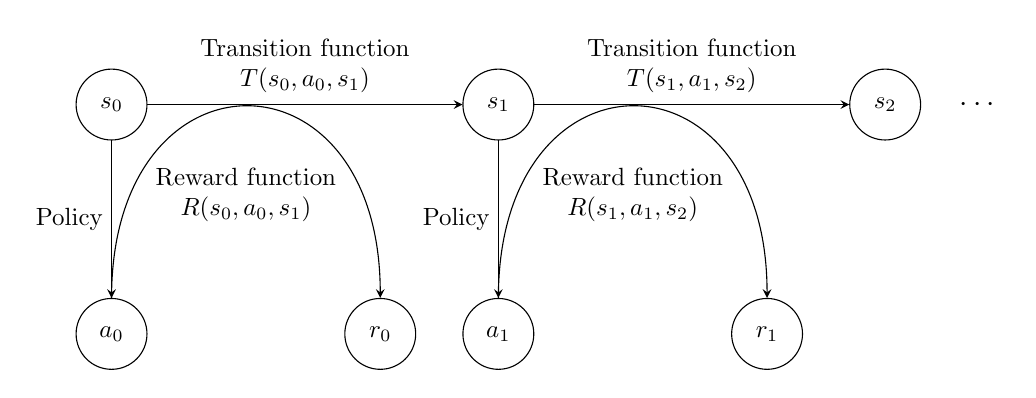
\begin{tikzpicture}[->, >=stealth, node distance=2cm, every node/.style={scale=0.9}]
    % State nodes
    \node[circle, draw, minimum size=1cm] (s0) {$s_0$};
    \node[circle, draw, minimum size=1cm, right=4cm of s0] (s1) {$s_1$};
    \node[circle, draw, minimum size=1cm, right=4cm of s1] (s2) {$s_2$};

    % Action nodes
    \node[circle, draw, minimum size=1cm, below=2cm of s0] (a0) {$a_0$};
    \node[circle, draw, minimum size=1cm, below=2cm of s1] (a1) {$a_1$};

    % Reward nodes
    \node[circle, draw, minimum size=1cm, right=2.5cm of a0] (r0) {$r_0$};
    \node[circle, draw, minimum size=1cm, right=2.5cm of a1] (r1) {$r_1$};

    % Arrows between states
    \draw[->] (s0) -- (s1) node[midway, above] {\begin{tabular}{c}
            Transition function \\
            $T(s_0, a_0, s_1)$
        \end{tabular}};
    \draw[->] (s1) -- (s2) node[midway, above] {\begin{tabular}{c}
            Transition function \\
            $T(s_1, a_1, s_2)$
        \end{tabular}};

    % Policy arrows 
    \draw[->] (s0) -- (a0) node[midway, left] {Policy};
    \draw[->] (s1) -- (a1) node[midway, left] {Policy};

    \draw[->] (a0) .. controls +(0,3.7) and +(0,3.7) .. node[midway, below, yshift=-20pt] {\begin{tabular}{c}
            Reward function \\
            $R(s_0, a_0, s_1)$
        \end{tabular}} (r0);

    \draw[->] (a1) .. controls +(0,3.7) and +(0,3.7) .. node[midway, below, yshift=-20pt] {\begin{tabular}{c}
            Reward function \\
            $R(s_1, a_1, s_2)$
        \end{tabular}} (r1);

    % Ellipsis
    \node at ($(s2)+(1.2cm,0)$) {\large $\cdots$};

\end{tikzpicture}
    \caption{Markov Decision Process with policy, transition, and reward functions}
    \label{fig:mdp}
\end{figure}

The agent's objective is to learn a policy $\pi: \mathcal{S} \rightarrow \mathcal{A}$ that maps states to actions, in order to maximise the expected cumulative reward over time. Policies can be categorised as:
\begin{itemize}
    \item deterministic: $\pi(s) : \mathcal{S} \to \mathcal{A}$, at a given state $s$, the policy specifies the only available action to take, or
    \item stochastic: $\pi(s, a) : \mathcal{S} \times \mathcal{A} \to [0, 1]$, at a given state $s$, the policy specifies the probability of taking action $a$.
\end{itemize}

\acrlong{mdp} are based on the idea that the current state is fully representative of the environment. However, in most real world scenarios, the agent does not have access to the complete state. In such cases, \acrfull{pomdp} can be used to model the uncertainty in the agent's observations and actions.

The goal of the agent is to maximise the cumulative long-term reward $G_t$, which is defined as the sum of discounted rewards over time:
\begin{equation}
    G_t = r_{t+1} + \gamma r_{t+2} + \gamma^2 r_{t+3} + \dots = r_{t+1} + \gamma G_{t+1}
\end{equation}
where $\gamma \in [0, 1)$ is the discount factor and is used to balance the importance between immediate and future rewards. If the discount factor is set to 0, the agent is myopic and only maximises the immediate reward; whereas, as $\gamma$ approaches $1$, the agent becomes more far-sighted and places greater importance on future rewards.

The expected cumulative reward is defined as the state value function $V^\pi(s): \mathcal{S} \to \mathbb{R}$, which is the expected return when starting from state $s$ and following policy $\pi$:
\begin{equation}
    V^\pi(s) = \mathbb{E}_\pi \left[G_t | s_t = s\right] 
\end{equation}
where $\mathbb{E}_\pi$ denotes the expectation over the policy $\pi$.

Similarly, the state-action value function $Q^\pi(s, a): \mathcal{S} \times \mathcal{A} \to \mathbb{R}$ is defined as the expected return when starting from state $s$, taking action $a$, and then following policy $\pi$:
\begin{equation}
    Q^\pi(s, a) = \mathbb{E}_\pi \left[G_t | s_t = s, a_t = a\right] 
\end{equation}

The state value function $V^\pi(s)$ and the state-action value function $Q^\pi(s, a)$ are related as follows:
\begin{equation}
    V^\pi(s) = \sum_{a \in \mathcal{A}} \pi(a | s) Q^\pi(s, a) = \mathbb{E}_\pi \left[Q^\pi(s, a) \mid s_t = s\right]
\end{equation}

Moreover, the advantage function $A^\pi(s, a)$ combines both the state value function $V^\pi(s)$ and the state-action value function $Q^\pi(s, a)$, and is defined as:
\begin{equation}
    A^\pi(s, a) = Q^\pi(s, a) - V^\pi(s)
\end{equation} 

A policy $\pi$ is said to be optimal if the policy's value function is the optimal value function of the \acrshort{mdp}, defined as: 
\begin{eqnarray}
    V^*(s) = \max_{\pi'} V^{\pi'}(s), \forall s \in \mathcal{S} \\ 
    Q^*(s, a) = \max_{\pi'} Q^{\pi'}(s, a), \forall s \in \mathcal{S}, a \in \mathcal{A}
\end{eqnarray}
The optimal policy $\pi^*$ is:
\begin{equation}
    \pi^*(s) = \arg \max_{a\in \mathcal{A}} Q^*(s, a)
\end{equation}

As a result, the optimal policy is the greedy policy that performs the optimal actions at each time step as determined by the optimal value functions. This framework enables the agent to determine optimal actions that maximise long-term returns by evaluating immediate information, without requiring knowledge of the values of future states and actions.

The \Gls{bellmanequations} \cite{Bellman1957book} provide a recursive relation between the value functions in terms of the future state/action values. There are four main Bellman equations, classified in two groups: the Bellman expectation equations and the Bellman optimality equations. The Bellman expectation equations are defined as follows:
\begin{eqnarray}
    V^\pi(s) = \sum_{a \in \mathcal{A}} \pi\left(a \mid s\right) \sum_{s'\in \mathcal{S}} T\left(s, a, s'\right) \left[R\left(s,a\right) + \gamma V^\pi(s')\right] \\ 
    Q^\pi(s, a) = \sum_{s'\in \mathcal{S}} T\left(s, a, s'\right) \left[R\left(s,a\right) + \gamma \sum_{a' \in \mathcal{A}} \pi\left(a' \mid s'\right) Q^\pi(s', a')\right]
\end{eqnarray}

and the Bellman optimality equations are defined as:
\begin{eqnarray}
    V^*(s) = \max_{a \in \mathcal{A}} \sum_{s'\in \mathcal{S}} T\left(s, a, s'\right) \left[R\left(s,a\right) + \gamma V^*(s')\right] \\
    Q^*(s, a) = \sum_{s'\in \mathcal{S}} T\left(s, a, s'\right) \left[R\left(s,a\right) + \gamma \max_{a' \in \mathcal{A}} Q^*(s', a')\right]
\end{eqnarray}

Although explicitly solving the Bellman equations would lead to the optimal policy, it is often intractable due to the size of the state and action spaces. Therefore, in \acrshort{rl} algorithms, the goal is to learn an approximation of the optimal value functions, which can be used to derive the optimal policy. Another problem that arises is that of balancing exploration and exploitation \cite{Thrun1992}. Theoretically, following the greedy action yields the optimal policy, but this is only true if all the action values are known. In practice, the agent at each time step and given state chooses either an action whose value is higher, thus exploiting its current knowledge, or picks an action at random, thus exploring the environment and gaining more information about the state-action space, leading to potentially discovering a better action than the greedy one at the current time.

\subsection{Deep Reinforcement Learning Algorithms} \label{sec:drlalgorithms}

A \acrlong{rl} agent includes one or more of the following components \cite{Francois-Lavet2018}:
\begin{itemize}
    \item a representation of the value function that provides a prediction of the value of each state or state-action pair,
    \item a direct representation of the policy $\pi$, and
    \item a model of the environment, consisting of estimates of transition and reward functions.
\end{itemize}

Depending on the components, the main \acrlong{rl} paradigms are: 
\begin{itemize}
    \item \textbf{Model-free} algorithms do not learn a representation of the environment, but focus on either the value function or the policy. 
    \begin{itemize}
        \item \textbf{Value-based} algorithms learn an approximation of the value function, which is used to compute the state or state-action values. The policy is not learnt explicitly but can be derived from the value function. Examples include \acrfull{dqn} \cite{Mnih2013} and C51 \cite{Bellemare2017}. 
        \item \textbf{Policy-based} algorithms learn a direct representation of the policy, which is used to select actions. \acrfull{a2c}, \acrfull{a3c} \cite{Mnih2016} and \acrfull{ppo} \cite{Schulman2017} are examples of policy-based algorithms.
        \item \textbf{Actor-Critic} algorithms combine both value-based and policy-based approaches, where the actor learns the policy and the critic learns the value function. The critic provides feedback to the actor to improve the policy. Some examples are \acrfull{ddpg} \cite{Lillicrap2015}, \acrfull{td3} \cite{Fujimoto2018}, and \acrfull{sac} \cite{Haarnoja2018}.
    \end{itemize}
    \item \textbf{Model-based} algorithms include a model of the environment, which can be used to simulate future states and rewards. For example, World Models \cite{HaGoogleBrainTokyo2018} learns a model of the environment and AlphaZero \cite{Silver2017} has a representation of the model. 
\end{itemize}

The taxonomy of the \acrshort{rl} algorithms is shown in Figure \ref{fig:rl_taxonomy}.
\begin{figure}[h]
    \centering
    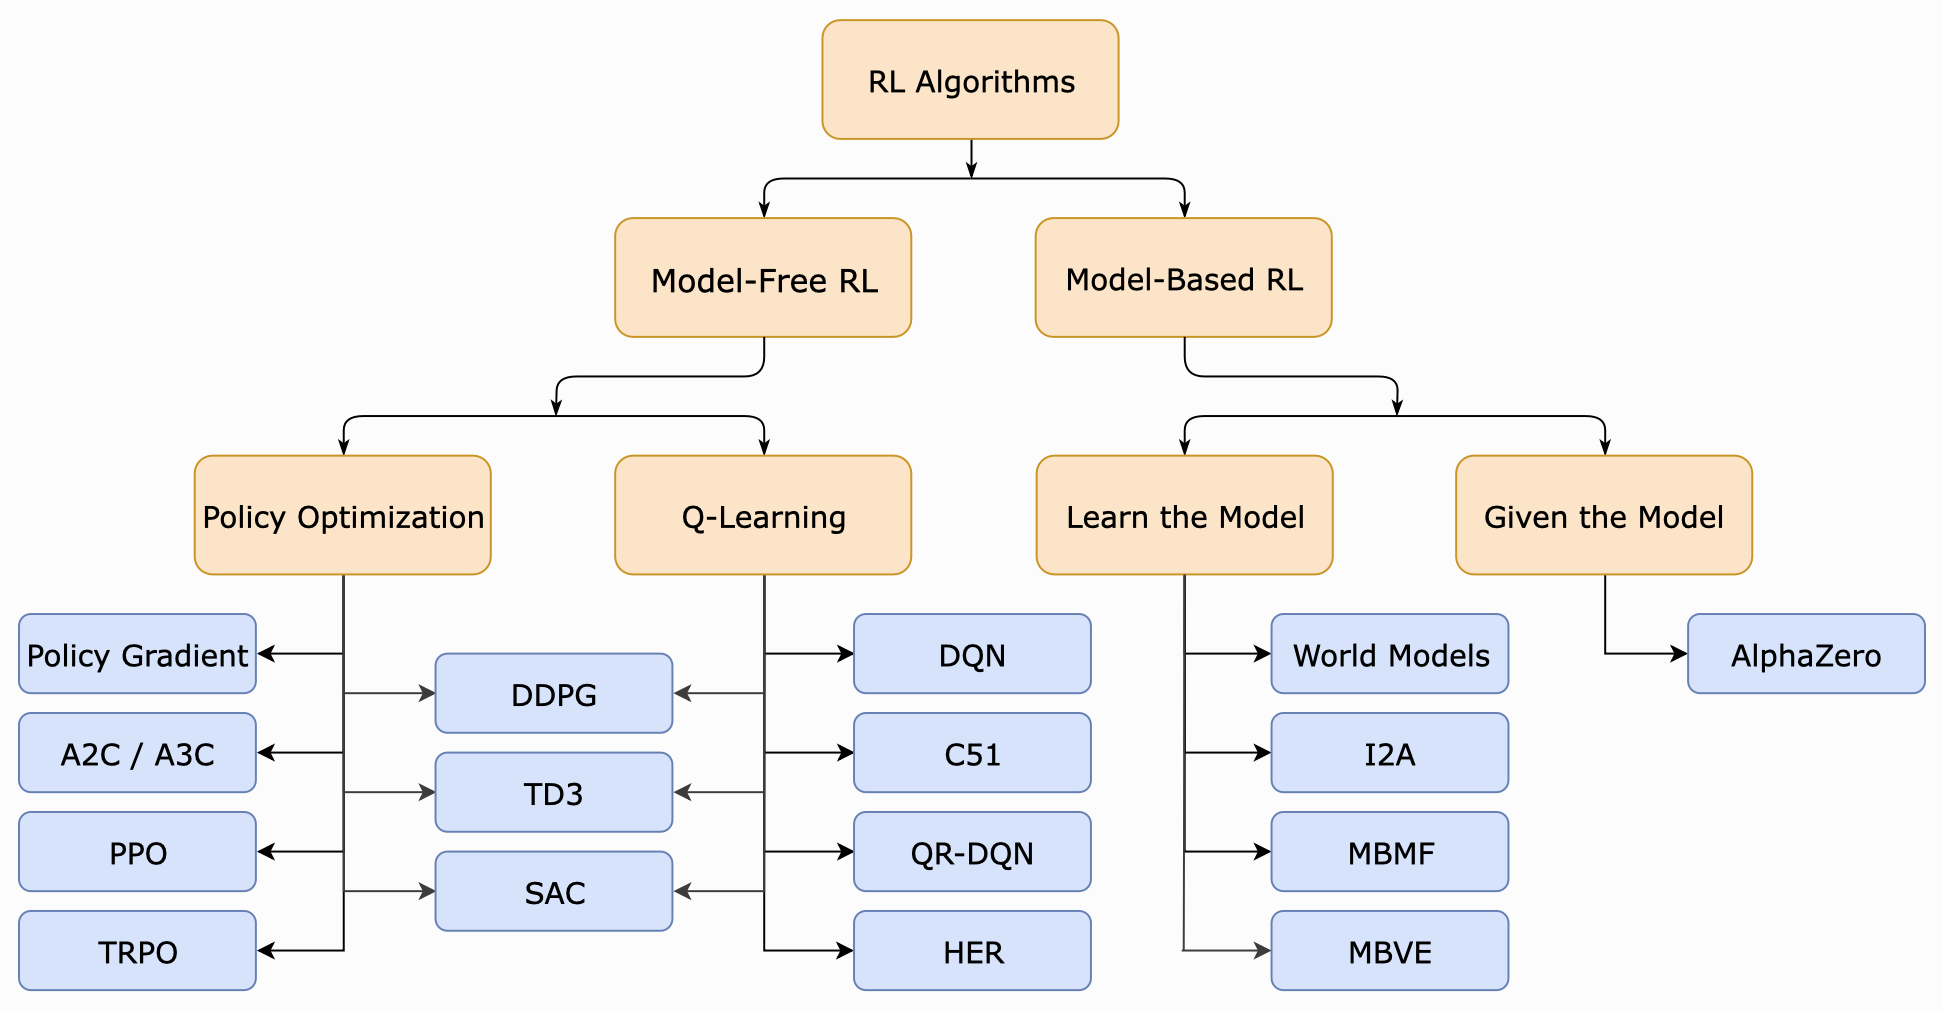
\includegraphics[width=0.8\textwidth]{figures/rl-taxonomy.png}
    \caption{Taxonomy of Reinforcement Learning Algorithms \cite{Achiam2018}}
    \label{fig:rl_taxonomy}
\end{figure}

The full potential of \acrlong{rl} algorithms is achieved when leveraging the power of \acrlong{dl} to solve dynamic stochastic control problems that have high-dimensionality in their representation of the state and action spaces. \acrshort{drl} algorithms use \acrshort{dnn}s to approximate the value functions, or use gradient ascent to find the optimal policy parameters. This thesis will focus on the following \acrshort{drl} algorithms on policy-based and actor-critic algorithms.

\subsubsection{Advantage Actor-Critic (A2C)} \label{sec:a2c}

The \acrfull{a2c} algorithm was developed by Mnih et al. (2016) in their paper on \textit{Asynchronous methods for deep reinforcement learning} \cite{Mnih2016}. The main contribution is the usage of the advantage function to address the variance issues present in policy gradient methods. The \acrshort{a2c} is the synchronous version of \acrshort{a3c}, and is preferred due to its better performance in terms of training time and cost-effectiveness \cite{Wu2017}.

The algorithm consists of a dual-network architecture, where the actor network learns a stochastic policy $\pi\left(a_t\mid s_t; \theta\right)$ and the critic network learns the value function $V\left(s_t; \theta_v\right)$. The policy and the value function are updated after every $t_max$ actions or when a terminal state is reached. The advantage function is estimated as follows: 
\begin{equation}
    A\left(s_t, a_t; \theta, \theta_v\right) = \sum_{i=0}^{k-1} \gamma^i r_{t+i} + \gamma^k V\left(s_{t+k}; \theta_v\right) - V\left(s_t; \theta_v\right)
\end{equation}
where $k$ represents the $n$-step return and is upper-bounded by the maximum number of steps $t_{max}$, and $\gamma$ is the discount factor. The algorithm's objective function is defined as:
\begin{equation}
    J\left(\theta, \theta_v\right) = \mathbb{E}_{\pi}\left[\log \pi\left(a_t\mid s_t; \theta\right) A\left(s_t, a_t; \theta, \theta_v\right)\right]
\end{equation}

The pseudo-code for the algorithm for \acrshort{a2c} is outlined in appendix \ref{alg:a2c}. 

\subsubsection{Proximal Policy Optimisation (PPO)} \label{sec:ppo}

\acrfull{ppo} is a policy gradient algorithm that was introduced by Schulman et al. (2017) in their paper on \textit{Proximal Policy Optimization Algorithms} \cite{Schulman2017} with the objective of constraining policy updates. The algorithm balances sufficiently large policy updates in order to improve the policy, while avoiding excessively large changes that could hinder performance. 

\acrshort{ppo} improves the performance of \acrfull{trpo} \cite{Schulman2015} by using a clipped surrogate objective function, by ensuring that the probability ratio $r_t$ is bounded within a range of $[1 - \epsilon, 1 + \epsilon]$, where $\epsilon$ is a hyperparameter that controls the clipping range. The objective function is defined as:
\begin{equation}
    L_t^{CLIP}(\theta) = \mathbb{E}_t \left[\min\left(r_t(\theta) \hat{A}_t, \text{clip}\left(r_t(\theta), 1 - \epsilon, 1 + \epsilon\right) \hat{A}_t\right)\right]
\end{equation}
where 
\begin{equation}
    r_t(\theta) = \frac{\pi_\theta(a_t | s_t)}{\pi_{\theta_{old}}(a_t | s_t)}
\end{equation}
is the probability ratio between the current policy $\pi_\theta$ and the old policy $\pi_{\theta_{old}}$

Another improvement with respect to \acrshort{trpo} is the use of simple first-order optimisation methods as opposed to the second-order methods used in \acrshort{trpo}. Consequently, \acrshort{ppo} maintains the stability and reliability of other trust-region methods, while being easier to implement and more computationally efficient. The pseudo-code for the algorithm for \acrshort{ppo} is outlined in appendix \ref{alg:ppo}.

\subsubsection{Deep Deterministic Policy Gradient (DDPG)} \label{sec:ddpg}

\acrfull{ddpg} is an off-policy actor-critic algorithm that was introduced by Lillicrap et al. (2015) in their paper on \textit{Continuous control with deep reinforcement learning} \cite{Lillicrap2015}. The algorithm arises to solve the challenges of applying \acrlong{dqn} \cite{Mnih2013} to continuous action spaces by applying \acrfull{dpg}, which enables the efficient computation of the policy gradient without the need to integrate over the action space. 

The algorithm uses the following networks: the actor network $\mu(s_t; \theta_\mu)$, which learns a deterministic policy, the critic network $Q(s_t, a_t; \theta_Q)$, which learns the state-action value function, and the actor's and critic's target networks. The actor network is updated using \acrshort{dpg}: 
\begin{equation}
    \nabla_{\theta_\mu} J \approx \mathbb{E}_{s_t \sim \mathcal{D}} \left[\nabla_a Q(s_t, a_t; \theta_Q) \nabla_{\theta_\mu} \mu(s_t; \theta_\mu)\right]
\end{equation}
where $\mathcal{D}$ is the replay buffer that stores the agent's experiences, and the critic network is updated using the \Gls{bellmanequations}:
\begin{equation}
    \nabla_{\theta_Q} J \approx \mathbb{E}_{s_t \sim \mathcal{D}} \left[\left(r_t + \gamma Q(s_{t+1}, \mu(s_{t+1}; \theta_\mu); \theta_Q') - Q(s_t, a_t; \theta_Q)\right) \nabla_{\theta_Q} Q(s_t, a_t; \theta_Q)\right]
\end{equation}
where $\theta_Q'$ are the parameters of the target critic network. 

From \acrlong{dqn}, the algorithm incorporates a replay buffer to store the agent's experiences, which allows the agent to learn from past experiences and improve its performance over time. Moreover, \acrshort{ddpg} incorporates noise, typically Ornstein-Uhlenbeck noise \cite{Uhlenbeck1930}, to the actions taken by the actor network to encourage exploration of the action space. The pseudo-code for the algorithm for \acrshort{ddpg} is outlined in appendix \ref{alg:ddpg}.

\subsubsection{Twin Delayed Deep Deterministic Policy Gradient (TD3)} \label{sec:td3}

\acrfull{td3} is an extension of \acrshort{ddpg} introduced by Fujimoto et al. (2018) in their paper on \textit{Addressing Function Approximation Error in Actor-Critic Methods} \cite{Fujimoto2018}. The proposal addresses the hyper-parameter sensitivity and overestimation bias present in the critic network of \acrshort{ddpg}. There are three main improvements to \acrshort{ddpg}:
\begin{itemize}
    \item \textbf{Clipped Double Q-Learning}: The algorithm employs two critic networks and uses their minimum value to compute the target value for the actor network, which reduces the overestimation bias. 
    \item \textbf{Delayed Policy Updates}: The actor and critic networks updates are performed at different frequencies. The critic networks are updated every time step, whereas the actor and target networks are updated less frequently. The main benefit is that it allows the critic to improve the accuracy of the value estimates before the actor updates its policy.
    \item \textbf{Target Policy Smoothing}: The algorithm adds noise to the target action during the critic updates to smooth the value function over similar actions, resulting in a lower impact of approximation errors and more robust policies. 
\end{itemize}

The pseudo-code for the algorithm for \acrshort{td3} is outlined in appendix \ref{alg:td3}.

\subsubsection{Soft Actor-Critic (SAC)} \label{sec:sac}

\acrfull{sac}, despite being an off-policy actor-critic algorithm, represents a paradigm shift in \acrshort{rl}. The algorithm was presented by Haarnoja et al. (2018) in their paper on \textit{Soft Actor-Critic: Off-Policy Maximum Entropy Deep Reinforcement Learning with a Stochastic Actor} \cite{Haarnoja2018} and is based on the maximum entropy framework, which aims to maximise both the expected return and the \gls{entropy} of the policy, encouraging the agent to succeed at the task while acting as randomly as possible. 

The algorithm uses two critic networks to estimate the state-action value function, and a stochastic actor network that learns a policy that maximises the expected return while also maximising the entropy of the policy. The critic networks are updated using the Bellman equations, and the actor network is updated using the policy gradient method. The objective function for the actor network is defined as:
\begin{equation}
    J(\theta) = \mathbb{E}_{s_t \sim \mathcal{D}} \left[\mathbb{E}_{a_t \sim \pi_\theta} \left[\alpha \log \pi_\theta(a_t | s_t) + Q(s_t, a_t; \theta_Q)\right]\right]
\end{equation}
where $\alpha$ is a temperature parameter that controls the trade-off between exploration and exploitation, and $\mathcal{D}$ is the replay buffer that stores the agent's experiences. The critic networks are updated using the Bellman equations:
\begin{equation}
    J(\theta_Q) = \mathbb{E}_{s_t \sim \mathcal{D}} \left[\left(r_t + \gamma \min_{i=1,2} Q(s_{t+1}, \mu_\theta(s_{t+1}) + \mathcal{N}(0, \sigma); \theta_{Q_i}) - Q(s_t, a_t; \theta_{Q_i})\right)^2\right]
\end{equation}
where $\mathcal{N}(0, \sigma)$ is the noise added to the action to encourage exploration, and $\theta_{Q_i}$ are the parameters of the two critic networks. The temperature parameter $\alpha$ is learned automatically by maximising the entropy of the policy, which is defined as:
\begin{equation}
    J(\alpha) = \mathbb{E}_{s_t \sim \mathcal{D}} \left[\alpha \log \pi_\theta(a_t | s_t)\right]
\end{equation}
This parameter is used to control the trade-off between the entropy and the reward terms, effectively controlling the stochasticity of the policy.

The pseudo-code for the algorithm for \acrshort{sac} is outlined in appendix \ref{alg:sac}.

\subsubsection{Algorithm comparison}

The five algorithms presented above are among the most widely used in the field of \acrshort{drl}, each addressing specific challenges in policy estimation and value function approximation. \acrshort{a2c} is an on-policy actor-critic method that reduces variance through advantage estimation, while \acrshort{ppo} changed on-policy learning by introducing a clipped surrogate objective that ensures stable policy updates. Although \acrshort{ddpg} pioneered continuous control through deterministic policies, \acrshort{td3} addressed the overestimation bias of its predecessor via twin critics and delayed updates. \acrshort{sac} revolutionised the field of \acrshort{drl} by incorporating maximum entropy principles.

An overview of the algorithms and their key characteristics is summarised in Table \ref{tab:drl_algorithms_comparison}. 

\begin{table}[h]
    \centering
    \begin{tabular}{|l|l|l|l|}
        \hline
        Algorithm & Policy Type & On/Off Policy & Key Idea \\
        \hline
        \acrshort{a2c} & Stochastic & On-Policy & Advantage Actor-Critic \\
        \acrshort{ppo} & Stochastic & On-Policy & Clipped Policy Updates \\
        \acrshort{ddpg} & Deterministic & Off-Policy & Actor-Critic + Replay buffer \\
        \acrshort{td3} & Deterministic & Off-Policy & Double critics + Delayed updates \\
        \acrshort{sac} & Stochastic & Off-Policy & Max-entropy \acrshort{rl} \\
        \hline
    \end{tabular}
    \caption{Comparison of Deep Reinforcement Learning Algorithms}
    \label{tab:drl_algorithms_comparison}
\end{table}

\section{Explainable Artificial Intelligence} \label{sec:explainableai}

\acrfull{xai} refers to a set of processes, methods and techniques that enable human users to comprehend and trust the outcomes and decisions made by \acrfull{ai} systems. The goal is to make \acrshort{ai} algorithms more transparent, interpretable, and accountable, allowing end-users to understand the outputs of the models. This is particularly important in \acrfull{dl} where the models are often considered black boxes  due to their complexity, non-linearity and high-dimensionality, making it difficult to understand how they arrive at their decisions. With explainable systems, the benefits are numerous ranging from informed decision making to increased user adoption and better governance \cite{Phillips2021}. 

Although there are many possible classifications of \acrshort{xai} methods, they can be broadly categorised into two main categories. First, transparent algorithms are inherently understandable and interpretable, such as linear regression, decision trees and rule-based systems. Second, post-hoc explanations are methods that require the usage of an additional algorithm to explain the decisions made by a model. Examples include saliency maps \cite{Sequeira2020} and interaction data \cite{Greydanus2018}. The post-hoc methods can be further sub-divided between global and local explanations. The goal of global explainability is to provide an understanding of the model's overall behaviour across the entire dataset, while local explainability focuses on explaining the individual predictions made by the model.

Another classification relates to whether the explanation method depends on the type of model it is being applied to. On the one hand, model-agnostic methods can be applied to any model regardless of its internal architecture, effectively treating all types of models as black boxes. The analysis is conducted by understanding the input-output behaviour and how small perturbations to the input impact the output. Examples include \acrfull{lime} \cite{Ribeiro2016} and \acrfull{shap} \cite{Lundberg2017}. On the other hand, model-specific methods are tailored to a particular architecture and leverage its components as part of the explanation process. In the case of neural networks, this can be achieved by analysing the learned features or by incorporating attention mechanisms \cite{Amirshahi2023}.

The taxonomy of the \acrshort{xai} methods is shown in Figure \ref{fig:xai_taxonomy}.
\begin{figure}[h]
    \centering
    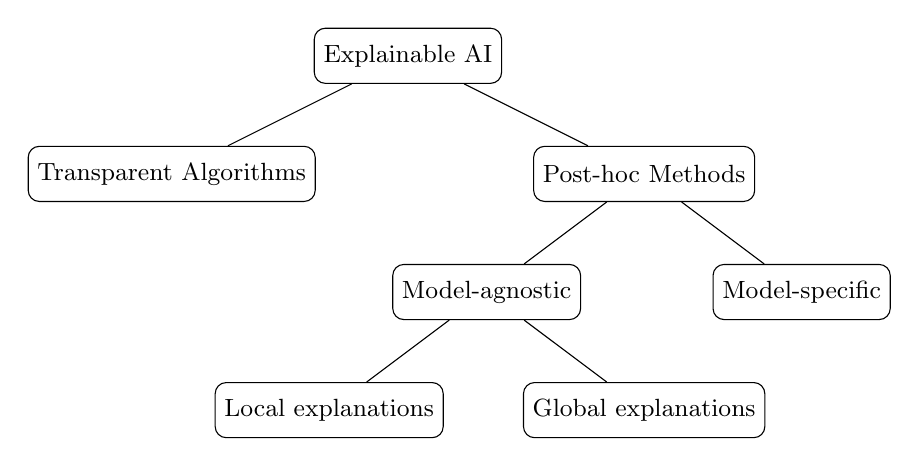
\begin{tikzpicture}[
  level 1/.style={sibling distance=60mm, level distance=15mm},
  level 2/.style={sibling distance=40mm, level distance=15mm},
  level 3/.style={sibling distance=40mm, level distance=15mm},
  every node/.style={rectangle, draw=black, rounded corners, align=center, font=\small, minimum height=0.7cm}
]

\node {Explainable AI}
  child {node {Transparent Algorithms}}
  child {node {Post-hoc Methods}
    child {node {Model-agnostic}
      child {node {Local explanations}}
      child {node {Global explanations}}
    }
    child {node {Model-specific}}
  };

\end{tikzpicture}

    \caption{Taxonomy of Explainable Artificial Intelligence Methods}
    \label{fig:xai_taxonomy}
\end{figure}

\subsection{Feature Importance} \label{sec:featureimportance}

\Gls{featureimportance} is a global model-specific method that quantifies the contribution of each feature to the model's predictions. In particular, permutation feature importance \cite{Breiman2001} measures the contribution of each feature by evaluating the model's performance on the original dataset and comparing it to the performance on a permuted version of the dataset, where a specific feature is randomly shuffled. The process allows to understand how much the model's relies on a particular feature for its prediction, by measuring the decrease in predictive power if the input feature's values vary.

An alternative method, well-suited for tree-based models, is impurity-based feature importance. Random forests split their features with the goal of reducing an impurity measure at each node, normally Gini impurity for classification tasks or mean squared error for regression. As such, a split with a large decrease of impurity is considered importance and as such the variable responsible for the split is considered important \cite{Nembrini2018}. As a result, the impurity importance of a feature is the sum of all impurity reductions across all nodes and trees in the forest where the particular feature was used to split the data. While powerful, this method suffers from bias towards features with high cardinality and they do not necessarily reflect the ability of a feature to make useful predictions on the test set, given that importance is computed on the training set. 

\subsection{Local Interpretable Model-agnostic Explanations (LIME)} \label{sec:lime}

\acrfull{lime} is a model-agnostic explanation method that explains individual predictions of a \acrlong{ml} model by analysing the model locally around the prediction of interest. The method, introduced by Ribeiro et al. (2016) in their paper on \textit{Why should I trust you? Explaining the predictions of any classifier} \cite{Ribeiro2016},utilises the black box model to understand what happens to the outputs when the input data is slightly modified, then fits a simpler, interpretable model to the perturbed data to approximate the black box model's behaviour in that local region.

Mathematically, let $\mathcal{L}(f,g,\pi_x)$ be a measure of how unfaithful an explanation model $g$ is in approximating the model $f:\mathbf{R}^d \to \mathbf{R}$ in the neighbourhood of the instance $x$ defined as $\pi_x$. The goal is to find an interpretable model $g \in G$ that minimises the following objective function:
\begin{equation}
    \xi(x) = \mathcal{L}(f, g, \pi_x) + \Omega(g)
\end{equation}
where $\Omega(g)$ is a regularisation term that penalises the complexity of the explanation model $g$. This encourages interpretability, meaning a qualitative understanding of the relationship between inputs and outputs and promotes local fidelity, ensuring the explanation accurately approximates the model's behaviour in the local region. 

The method works as follows:
\begin{itemize}
    \item \textbf{Instance Selection}: Start with a specific prediction instance that requires explanation.
    \item \textbf{Perturbation}: Generate synthetic data points by perturbing the original instance.
    \item \textbf{Model Querying}: Obtain predictions from the black-box model for these perturbed instances.
    \item \textbf{Weighting}: Assign weights to the synthetic data points based on their proximity to the original instance.
    \item \textbf{Surrogate Training}: Train a simple, interpretable model (typically linear regression) on the weighted synthetic dataset.
    \item \textbf{Explanation}: Use the surrogate model to explain the original prediction by interpreting its coefficients or structure.
\end{itemize}

Its main advantages are its ability to work across different types of data and models, due to its model-agnostic nature, and the fact that its explanations are human-friendly and include a fidelity measure that indicates how well the explanation approximates the black-box model's local behaviour. Nonetheless, the method offers only local explanations, which may not generalise well to the entire model; it relies on the choice of neighbourhood; and the complexity of the surrogate model needs to be defined in advance and can compromise the interpretability of the explanation \cite{Molnar2025}.

\subsection{SHapley Additive exPlanations (SHAP)} \label{sec:shap}

Another model-agnostic technique is \acrfull{shap}, which was introduced by Lundberg and Lee (2017) in their paper on \textit{A unified approach to interpreting model predictions} \cite{Lundberg2017}. The method is based on cooperative game theory and the concept of Shapley values \cite{Shapley1953}.

The Shapley value arises in cooperative game theory to answer the question of how to fairly distribute the contribution of each player in a coalition. In this framework, a coalitional game is represented as a tuple $(N,v)$, where $N = \{1, 2, \ldots, n\}$ is the set of players and $v: 2^N \rightarrow \mathbb{R}$ is the characteristic function that assigns a value $v(S)$ to each possible coalition $S \subseteq N$, with the convention that $v(\emptyset) = 0$. The characteristic function $v(S)$ represents the total value that coalition $S$ can achieve through cooperation. 

Mathematically, the Shapley value for a feature $i$ is defined as:
\begin{equation}
    \phi_i = \sum_{S \subseteq N \setminus \{i\}} \frac{|S|! (|N| - |S| - 1)!}{|N|!} \left[ v_{S \cup \{i\}}(x_{S \cup \{i\}}) - v_S(x_S) \right]
\end{equation}
where $S \subseteq N$ is a subset of all features $N$, $v_{S \cup \{i\}}$ is marginal contribution of player $i$ to coalition $S$, and $v_S$ is the value of coalition $S$ without player $i$. This formula can be understood as computing the weighted average of marginal contributions of feature $i$ across all possible coalitions. 

The advantage of Shapley values is that it is the only attribution method that results in a fair payout. In particular, it satisfies the four fundamental properties that define a fair allocation: 

\begin{itemize}
    \item \textbf{Efficiency:} The sum of all Shapley values equals the value of the grand coalition:
    \[
        \sum_{i \in N} \phi_i = v(N)
    \]
    \item \textbf{Symmetry:} The contributions of two players $i$ and $j$ should be equal if they make identical marginal contributions to all possible coalitions:
    \[
        v(S \cup \{i\}) = v(S \cup \{j\}), \forall S \subseteq N \setminus \{i, j\} \implies \phi_i = \phi_j
    \]
    \item \textbf{Dummy:} If a player contributes nothing to any coalition they join, their Shapley value should be zero:
    \[
        v(S \cup \{i\}) = v(S), \forall S \subseteq N \setminus \{i\} \implies \phi_i = 0
    \]
    \item \textbf{Additivity:} For two games $(N,v_1)$ and $(N,v_2)$, the Shapley value of the combined game $(N,v_1+v_2)$ equals the sum of individual Shapley values:
    \[
        \phi_i(v_1 + v_2) = \phi_i(v_1) + \phi_i(v_2)
    \]
\end{itemize}

The algorithm for approximating Shapley values is outlined in \ref{alg:shapley}. However, the method is computationally expensive, as it requires evaluating the model for all possible coalitions of features.

\begin{algorithm}
\caption{Shapley Value Approximation}
\begin{algorithmic}
\State \textbf{Initialise:} 
\State Number of iterations $M$
\State Instance of interest $\mathbf{x}$
\State Feature index $j$
\State Data matrix $\mathbf{X}$
\State Model $\hat{f}$

\For{$m = 1$ to $M$}
    \State Draw a random instance $\mathbf{z}$ from data matrix $\mathbf{X}$
    \State Choose a random permutation $\mathbf{o}$ of the feature indices
    \State Order $\mathbf{x}$ according to $\mathbf{o}$: $\mathbf{x}_{\mathbf{o}} = \left(x_{(1)}, \dots, x_{(j)}, \dots, x_{(p)}\right)$
    \State Order $\mathbf{z}$ according to $\mathbf{o}$: $\mathbf{z}_{\mathbf{o}} = \left(z_{(1)}, \dots, z_{(j)}, \dots, z_{(p)}\right)$
    
    \State Construct two new instances:
    \State \hskip1.5em $\mathbf{x}_{+j} = \left(x_{(1)}, \dots, x_{(j-1)}, x_{(j)}, z_{(j+1)}, \dots, z_{(p)}\right)$
    \State \hskip1.5em $\mathbf{x}_{-j} = \left(x_{(1)}, \dots, x_{(j-1)}, z_{(j)}, z_{(j+1)}, \dots, z_{(p)}\right)$
    
    \State Compute marginal contribution: 
    \[
        \phi_j^{(m)} = \hat{f}(\mathbf{x}_{+j}) - \hat{f}(\mathbf{x}_{-j})
    \]
\EndFor

\State Compute average Shapley value:
\[
    \phi_j(\mathbf{x}) = \frac{1}{M} \sum_{m=1}^M \phi_j^{(m)}
\]

\end{algorithmic}
\label{alg:shapley}
\end{algorithm}

The use of Shapley values in \acrshort{ml} was not introduced until 2011, when Štrumbelj and Kononenko \cite{Strumbelj2011} proposed it as a method for explaining black-box regression models. However, it was popularised in 2017 by Lundberg and Lee \cite{Lundberg2017}, who introduced the \acrshort{shap} framework. Although their proposal relies on the principles of Shapley values, their main contribution is to represent the Shapley value as an additive feature attribution method. The explanation is given as:
\begin{equation}
    g(\mathbf{z}') = \phi_0 + \sum_{i=1}^{M} \phi_j z'_j
\end{equation}
where $g$ is the explanation model, $\mathbf{z}' \in \{0,1\}^M$ is the coalition vector, $M$ is the maximum coalition size and $\phi_j$ is the feature attribution for feature $j$.

\subsubsection{KernelSHAP} \label{sec:kernelshap}

The KernelSHAP algorithm builds on the \acrshort{shap} framework by using a kernel-based approach to estimate Shapley values. It approximates the Shapley value by sampling different coalitions and using a weighted linear regression model to fit the contributions of each feature. The method relies on not all coalitions contributing equally to the final Shapley value and as such uses kernel weights to identify the most important coalitions. The main steps of the KernelSHAP algorithm are:
\begin{itemize}
    \item Sample a set of coalitions from the feature space: $\mathbf{z}'_k \in \{0,1\}^M, k \in \{1, \ldots, K\}$, where $K$ is the total number of samples.
    \item For each coalition $\mathbf{z}'_k$, compute the model's prediction by first converting $\mathbf{z}'_k$ to the original feature space and then applying the model $\hat{f}$ : $\hat{f}\left(h_\mathbf{x}\left(\mathbf{z}'_k\right)\right)$.
    \item Compute the weight for each coalition with the SHAP kernel: $\pi_\mathbf{x} (\mathbf{z}')$ 
    \item Fit a weighted linear regression model to the sampled coalitions and their corresponding predictions.
    \item Return shapley values $\phi_k$ as the coefficients of the fitted model.
\end{itemize}

The sample coalitions are generated by randomly selecting subsets of the features, or equivalently, a vector of 0s and 1s indicating whether a feature is included in the coalition or not. The sampled coalitions represent the dataset for the regression model whose target is the prediction for a coalition. However, the sampled coalitions are not on the target feature space and, as such, it is necessary to implement another function $h_{\mathbf{x}}\left(\mathbf{z}'\right) = \mathbf{z}$ that maps the sampled coalitions to the original feature space. In the case of tabular data, this is done by replacing the features that are not included in the coalition with their mean value or a random sample from its possible values. As a result, sampling from the marginal distribution ignores the dependence structure between features.

Although there are similarities between \acrshort{shap} and \acrshort{lime}, their main difference lies in feature weighting in the regression model. The \acrshort{shap} weighting assumes that small and large coalitions provide the most information about its isolated effects or a its total effects, respectively. Whereas coalitions with half the features add little information about a specific feature contributions. The proposed weighting function for KernelSHAP is:
\begin{equation}
    \pi_\mathbf{x} (\mathbf{z}') = \frac{(M - 1)}{\binom{M}{|\mathbf{z}'|} |\mathbf{z}'| \left(M - |\mathbf{z}'|\right)}
\end{equation}
where $M$ is the maximum coalition size and $|\mathbf{z}'|$ is the number of features in the coalition $\mathbf{z}'$.

In addition, since the coalitions with the smallest and the largest number of features are the most informative, the sampling process is biased towards coalitions of size $1$ and $M-1$, resulting in $2M$ possible coalitions. Then, the remaining budget $K - 2M$ is used to sample coalitions of size $2$ to $M-2$. This process continues until the sampled coalitions reach the desired number of samples $K$.

Consequently, given the samples, the KernelSHAP algorithm fits a weighted linear regression model to estimate the Shapley values. The model is defined as:
\begin{equation}
    g(\mathbf{z}') = \phi_0 + \sum_{j=1}^{M} \phi_j z'_j
\end{equation}

The goal is to minimise the following loss function:
\begin{equation}
    \mathcal{L}(\hat{f}, g, \pi_{\mathbf{x}}) = \sum_{\mathbf{z}' \in \mathcal{Z}} \left[\hat{f} \left(h_{\mathbf{x}}\left(\mathbf{z}'\right)\right) - g(\mathbf{z}')\right]^2 \pi_{\mathbf{x}}(\mathbf{z}')
\end{equation}
where $\mathbf{Z}$ is the dataset of sampled coalitions. 

\chapter{Methodology} \label{ch:methodology}

This chapter covers the methodology and framework established to provide an explainable \acrfull{drl} model capable of optimising a portfolio of financial assets. The chapter is structured as follows: first, it describes the architecture and components of the proposed \acrshort{drl} model, including the state representation, reward function and training process. Second, it discusses the evaluation metrics and experimental setup used to assess the performance of the proposed solution. Finally, it outlines the implementation of the explainability techniques used to interpret the model's decisions. 

\section{Problem Definition} \label{sec:problem-definition}

The problem of \gls{portfoliooptimisation} is the task of finding an optimal allocation of financial assets in a portfolio to maximise expected returns while minimising risk. Thus, it is necessary to decide how to rebalance the portfolio at each time step in a highly stochastic and complex financial market. This can be formulated using a \acrfull{mdp} framework, where the agent interacts with the environment by deciding the optimal allocation based on the state of the environment at each time step to maximise the expected cumulative reward over time. \acrfull{drl} gives the agent the ability to learn the optimal policy directly from the environment by taking actions and receiving rewards. 

\section{Markov Decision Process Model} \label{sec:mdp-model}

Due to the dynamic, stochastic and interactive nature of financial markets, a \acrlong{mdp} is a suitable framework to model the problem. The main elements of the \acrshort{mdp} model are defined as follows:
\begin{itemize}
    \item State space $\mathcal{S}$
    \item Action space $\mathcal{A}$
    \item Reward function $R: \mathcal{S} \times \mathcal{A} \times \mathcal{S} \to \mathbb{R}$
    \item Transition function $T: \mathcal{S} \times \mathcal{A} \to \mathcal{S}$
    \item Discount factor $\gamma \in [0,1]$
\end{itemize}

The state space $\mathcal{S}$ is a vector representation of the financial environment. For a portfolio of $D$ assets, the features that describe the state include asset prices, technical indicators and macroeconomic indicators: 
\begin{itemize}
    \item Close price $\mathbf{p}_t \in \mathbb{R}^D$: Adjusted close prices of the assets at time $t$.
    \item Open price $\mathbf{o}_t \in \mathbb{R}^D$: Opening prices of the assets at time $t$.
    \item High price $\mathbf{h}_t \in \mathbb{R}^D$: Highest prices of the assets at time $t$.
    \item Low price $\mathbf{l}_t \in \mathbb{R}^D$: Lowest prices of the assets at time $t$.
    \item Volume $\mathbf{v}_t \in \mathbb{R}^D$: Trading volume of the assets at time $t$.
    \item Technical indicators $\mathbf{I}_t \in \mathbb{R}^{D \times I}$: For each of the $D$ assets, a vector $\mathbf{i}_t$ of $I$ technical indicators, such as moving averages, relative strength index (RSI), and Bollinger Bands, calculated from the asset prices.
    \item Macroeconomic indicators $\mathbf{M}_t \in \mathbb{R}^{D \times M}$: For each of the $D$ assets, a vector $\mathbf{m}_t$ of $M$ macroeconomic indicators, such as volatility index and interest rates, which provide additional context about the financial environment.
    \item Covariance matrix $\mathbf{C}_t \in \mathbb{R}^{D \times D}$: For each of the $D$ assets, a vector of $D$ values representing the covariance between the assets in the portfolio at time $t$.
\end{itemize}

The description of technical and macroeconomic indicators is provided in more detail in Appendix \ref{app:state_representation}.

The action space $\mathcal{A}$ is the set of possible actions that the agent can take at each time step. For the portfolio optimisation problem, the actions correspond to portfolio weights and are defined as follows:
\begin{equation}
    \mathbf{a}_t = \mathbf{w}_t : w_{t,d} \in [0, 1] \quad \forall d \in \{1, \ldots, D\},
\end{equation}
where $\mathbf{w}_t$ is a vector of portfolio weights at time $t$, representing the allocation of the portfolio to each asset. The weights are constrained to be non-negative and sum to one:
\begin{equation}
    \sum_{d=1}^D w_{t,d} = 1, \quad w_{t,d} \geq 0 \quad \forall d \in \{1, \ldots, D\}.
\end{equation}
Moreover, they are initialised to be equal for all assets, meaning that the agent starts with an equal allocation to each asset in the portfolio. The reason behind this is to avoid an initial bias and allow the agent to learn an allocation from the environment rather than favour any particular asset.

The transition function $T$ describes how the state of the environment changes in response to the action taken. It is defined as:
\begin{equation}
    s_{t+1} = T(s_t, a_t),
\end{equation}
where $s_{t+1}$ is the new state of the environment after taking action $a_t$ in state $s_t$. The transition function is determined by the dynamics of the financial market, which are influenced by the asset prices, trading volume and other factors.

The reward function $R$ models the direct reward of taking an action $a_t$ in state $s_t$ and transitioning to a new state $s_{t+1}$. It is defined as the change in the portfolio value from time $t$ to time $t+1$:
\begin{equation}
    R_{t+1} = R(s_t, a_t, s_{t+1}) = V_{t+1} - V_t,
\end{equation}
where the value of the portfolio at time $t$ is given by the dot product of the portfolio weights and the asset close prices:
\begin{equation}
    V_t = \mathbf{w}_t \cdot \mathbf{p}_t.
\end{equation}

An alternative formulation of the reward function is to use the Sharpe ratio \cite{Sharpe1994}, which is defined as the ratio of the expected return to the standard deviation of the returns:
\begin{equation}
    R(s_t, a_t, s_{t+1}) = \frac{E[r_{t+1}]}{\sigma[r_{t+1}]},
\end{equation}
where $E[r_{t+1}]$ is the expected return of the portfolio at time $t+1$ and $\sigma[r_{t+1}]$ is the standard deviation of the returns at time $t+1$. This formulation encourages the agent to maximise the expected return while minimising the risk of the portfolio.

Regardless of the choice of reward function, the goal of the agent is to learn a policy $\pi: \mathcal{S} \to \mathcal{A}$ that maximises the expected cumulative reward over time, which can be expressed as:
\begin{equation}
    J(\pi) = \mathbb{E} \left[\sum_{t=0}^{T} \gamma^t R(s_t, a_t, s_{t+1}) \right],
\end{equation} 
where $T$ is the time horizon and $\gamma$ is the discount factor that determines the importance of future rewards. 

The environment is implemented in \Gls{python} \footnote{https://www.python.org/} using the \texttt{Gym} library \cite{Brockman2016}, which provides a standard interface for reinforcement learning environments. The environment is defined as a class that inherits from the \texttt{gym.Env} class and implements the required methods: \texttt{reset}, \texttt{step} and \texttt{render}.

\section{Deep Reinforcement Learning Algorithms} \label{sec:drl-algorithms}

The proposed solution is based on the \acrshort{drl} framework, which allows the agent to learn the optimal policy directly from the environment by taking actions and receiving rewards. The algorithms used are:
\begin{itemize}
    \item \acrfull{a2c}
    \item \acrfull{ppo}
    \item \acrfull{ddpg}
    \item \acrfull{td3}
    \item \acrfull{sac}
\end{itemize}

The implementation is done using the \texttt{Stable Baselines3} library \cite{Raffin2021}, which provides a set of state-of-the-art \acrshort{drl} algorithms with a consistent interface and easy-to-use API. The pseudo-code for each algorithm is provided in Appendix \ref{app:drl_algorithms}.

\subsection{Hyper-parameter tuning} \label{subsec:hyperparameter-tuning}

Hyper-parameter tuning is a crucial step in the training process of \acrshort{drl} models, as the right choice of hyper-parameters can significantly impact the model's performance. In this thesis, hyper-parameter tuning refers to the process of optimising the training parameters of the \acrshort{drl} algorithms to maximise their performance in the task of portfolio optimisation. The hyper-parameters tuned include the learning rate, batch size, number of training steps, and other algorithm-specific parameters, which are summarised in Appendix \ref{app:hyperparameter_tuning}. 

To implement hyper-parameter tuning in Python, the \texttt{wandb} \cite{wandb} library is used, which provides a simple and efficient way to track experiments, visualise results, and manage hyper-parameter sweeps. A sweep is defined as a search for hyper-parameters that optimises a cost function, in our case, the Sharpe ratio. Given that the models were implemented using the \texttt{Stable Baselines3} library, the integration with \texttt{wandb} allows for seamless tracking of hyper-parameter configurations and their corresponding performance metrics \cite{WeightsBiases2025}.

As mentioned above, sweeps can optimise a cost function to avoid naively testing every possible combination. Using \texttt{wandb}, a Bayesian optimisation approach is taken \cite{Falkner2018}, which uses a probabilistic model to estimate the performance of different hyper-parameter configurations and selects the next configuration to test based on the expected improvement over the current best configuration. This allows for a more efficient search of the hyper-parameter space and reduces the number of configurations that need to be tested. Another option to reduce the time taken to find the optimal hyper-parameters is to use early termination. This method will stop a poorly performing run before it has fully completed, saving computational resources.

\section{Post-hoc Explainability} \label{sec:post_hoc_explainability}

Given the goal of improving the explainability of the \acrshort{drl} models, this thesis adopts explainability techniques to interpret the model's decision-making process in a transparent manner. By using post-hoc methods, rather than modifying each model's architecture to enhance their transparency, the proposal is model-agnostic and can be applied to any \acrshort{drl} model. Consequently, it combines the ability to find the most suitable architecture while maintaining the interpretability.

The explainability techniques implemented are: 
\begin{itemize}
    \item \Gls{featureimportance}
    \item \acrfull{lime}
    \item \acrfull{shap}
\end{itemize}

Following the work from de-la-Rica-Escudero et al. (2025) \cite{de-La-Rica-Escudero2025}, the implementation of these techniques follows two directions. First, as in their paper, a surrogate model maps the state space to the action space as a proxy for the model's decisions. The second direction is to use the \acrshort{lime} and \acrshort{shap} techniques directly on the \acrshort{drl} model to interpret its decisions.

\subsection{Surrogate Model Explainability} \label{subsec:surrogate_model_explainability}

The surrogate model is trained to approximate the behaviour of the \acrshort{drl} model by learning the mapping from its inputs, the environment representation, to its outputs, the portfolio weights. In the paper \cite{de-La-Rica-Escudero2025}, the authors do not explicitly acknowledge the use of a surrogate model, even though their code implementation does so. A potential reason behind not explaining the model's actions directly could be the code complexity in using \acrshort{shap} with a \acrshort{dl} model. 

Given that the action space is continuous, the surrogate model is implemented using a \texttt{RandomForestRegressor} \cite{sklearnRandomForest}, which is a non-parametric model that can capture complex relationships between the inputs and outputs. The model is trained on the state-actions pairs of the test data, which is the object of the explanations. However, since the model has a number of hyper-parameters, it requires careful tuning to achieve optimal performance. Consequently, hyperparameter tuning was used find the optimal architecture using \texttt{HalvingGridSearchCV} \cite{sklearnHalvingGridSearch}, which is a method that iteratively narrows down the search space by evaluating a subset of hyper-parameters and discarding the less promising ones. The use of grid search rather than Bayesian Optimisation, as was done for \acrshort{drl} hyper-parameter tuning \ref{subsec:hyperparameter-tuning}, is to replicate the approach taken in \cite{de-La-Rica-Escudero2025}. Once the optimal hyper-parameters have been found and the surrogate model has been trained, its prediction function is used as a proxy to interpret the original model's decisions.

Firstly, feature importance is built-in for Random Forest Regressors, and can be easily accessed with the built-in property \texttt{feature\_importances\_} \cite{sklearnFeatureImportance}. This method provides the importance of each feature in the state representation by using a combination of the fraction of the samples a feature contributes to and the mean decrease in impurity.

Secondly, \acrshort{lime} and \acrshort{shap} are applied to the surrogate model via the predict function to provide local explanations for individual predictions. Both of these techniques provide insights into the model's decisions by perturbing the input data and observing the changes in the output. 

The \acrshort{lime} implementation is done using the \texttt{LimeTabularExplainer} \cite{LimeTabularExplainer}, which is designed to work with tabular data and provides a way to explain individual predictions by approximating the model's behaviour locally with a linear model. Similarly, for \acrshort{shap}, the framework provides a particular implementation for tree-based models, which is used to compute the \acrshort{shap} values efficiently by exploiting the structure of the trees. Consequently, the \texttt{TreeExplainer} \cite{ShapTreeExplainer} is used to compute the \acrshort{shap} values for the surrogate model.

\subsection{Direct Model Explainability} \label{subsec:direct_model_explainability}

Undoubtedly, a surrogate model adds an additional layer of complexity and may obscure the understanding of the original model's decisions. Therefore, the \acrshort{lime} and \acrshort{shap} techniques are also applied directly to the prediction function of \acrshort{drl} model. This approach allows for a more direct interpretation of the model's decision-making process, without the need of a supplementary level. 

For \acrshort{lime}, the implementation is again done using \texttt{LimeTabularExplainer}, but the prediction function is now obtained from the relevant \acrshort{drl} algorithm. For \acrshort{shap}, the \texttt{KernelExplainer} is used, which is a model-agnostic method that randomly samples feature coalitions to approximate \acrshort{shap} values to reduce computation \cite{ShapKernelExplainer}.

\chapter{Results} \label{ch:results}

This chapter presents the results of conducting experiments under the methodology proposed in Chapter \ref{ch:methodology}. The experiments were designed to evaluate the performance of the implemented \acrshort{drl} models for portfolio optimisation in changing environment representations and market conditions. Moreover, to enable the interpretability of the model's decisions, a framework using post-hoc explainability techniques is explored.

\section{Dataset} \label{sec:dataset}

Given the general difficulty in finding the appropriate \acrshort{drl} algorithm with a suitable \gls{rewardfunction} for portfolio optimisation, the five implemented algorithms were tested on five different datasets. Each dataset consists of a different set of financial assets, ranging from three different asset classes. First, three datasets were constructed using the stock constituents of three renowned indexes:
\begin{itemize}
    \item \acrfull{djia} with 30 stocks,
    \item \acrfull{eurostoxx50} with 50 stocks, and
    \item \acrfull{ftse100} with 100 stocks.
\end{itemize}

The constituents of each of the indexes were retrieved in April 2025 and can be found in Appendix \ref{sec:datasets-equities}. It is important to note that the datasets were chosen to illustrate different currencies, as this introduces another factor of changing market conditions. 

Additionally, two datasets were constructed using commodities and currencies, respectively. The commodities dataset includes six different commodities, which are listed in Appendix \ref{sec:datasets-commodities}. These are a sample of the most traded commodities in the market and were chosen by their availability in the \texttt{Yahoo! Finance API} \footnote{https://uk.finance.yahoo.com}. With regard to the currencies dataset, it includes ten different currency pairs, listed in Appendix \ref{sec:datasets-currencies}. These were selected based on their trading volume and liquidity, with all pairs quoted in \acrfull{usd}.

The datasets are constructed using daily data from January 2016 to July 2025 downloaded using the Python \texttt{yfinance} library \cite{yfinance}. The dataset is partitioned into two disjoint sets: training and testing, with the training set containing data from January 2016 to December 2023, and the testing set starting on January 2024 until July 2025. For hyper-parameter tuning, the training set is further split into a training and validation set, with the validation sets corresponding to the period between January 2023 and December 2023. 

\section{Experiment Design} \label{sec:experiment-design}

To address the challenge of finding a suitable algorithm for portfolio optimisation, the five implemented \acrshort{drl} algorithms were tested on the five datasets described in Section \ref{sec:dataset}, with the goal of evaluating the performance of each algorithm in different scenarios and market conditions. Moreover, the environment representation will also be varied to assess the impact of more information on the model's performance. Four environment representations were considered, each with a different number of features.
\begin{itemize}
    \item Simple dataset: \acrfull{ohlcv} of the assets.
    \item Covariance dataset: To the simple dataset, the covariance matrix of the assets is added to explicitly model the relationships between the assets.
    \item Indicators dataset: Technical and macroeconomic indicators are added to the simple dataset.
    \item Complete dataset: The complete dataset includes the \acrshort{ohlcv}, the covariance matrix and the technical and macroeconomic indicators.
\end{itemize}

The strength of \acrshort{drl} algorithms lies in their ability to learn from high-dimensional data, which is why the goal is to evaluate whether a more exhaustive environment representation leads to better performance, despite the higher computational cost.

Finally, the performance of the algorithms is closely related to the choice of hyper-parameters. Ideally, the hyper-parameters should be tuned to find the optimal configuration for each algorithm and dataset combination. However, it was not feasible to perform tuning for all combinations of algorithms, datasets and environment representations. Consequently, the default hyper-parameters for all the experiments were chosen based on a testing run that was done on a small dataset of five tickers with indicators as environment representation. Those results can be seen in Appendix \ref{app:experiment_hyperparameters} and the default hyper-parameters are summarised in Appendix \ref{app:default_hyperparameters}.

Overall, the experiments were designed to evaluate the performance of the implemented \acrshort{drl} algorithms in different scenarios, with the goal of finding the most suitable algorithm for portfolio optimisation. However, testing five algorithms on five distinct datasets with four possible environment representations would result in a total of twenty different experiments per algorithm. Additionally, optimising the parameters for each experiment further expands the experimental space and significantly increases the computational time required. 

Due to limited computational resources\footnote{The university did not provide access to a computing cluster; therefore, all experiments were conducted on a personal computer.}, the scope of experiments was adjusted as follows. Firstly, hyper-parameter tuning was performed only for the Dow Jones 30 dataset with simple and indicators environment representation, as it is the smallest equities dataset and requires less computational time. Second, since the covariance matrix increases the dimensionality of the environment representation, it was only included in the experiments with the Dow Jones 30, the currencies and the commodities datasets.
\section{Evaluation} \label{sec:evaluation}

As outlined in the previous section, the experiments are designed to evaluate the performance of the implemented \acrshort{drl} algorithms in different scenarios and market conditions. The evaluation will focus on key performance metrics, as well as benchmarking against traditional portfolio optimisation techniques.

\subsection{Performance Metrics} \label{sec:performance-metrics}

The performance metrics are provided through the \texttt{pyfolio} library \cite{pyfolio}, which includes a \texttt{perf\_stats} method to calculate various performance metrics of a strategy. 

The main metrics for comparison are:
\begin{itemize}
    \item The cumulative return is the total change in investment price over a period of time, representing the overall percentage gain or loss from the initial investment value. The formula is given by:
    \begin{equation}
        \text{Cumulative return} = \frac{\text{Final portfolio value} - \text{Initial portfolio value}}{\text{Initial portfolio value}}.
    \end{equation}
    \item The annualised return is the geometric average of the amount of money earned by an investment each year over a given period of time, providing a standardised measure of annual performance. It is calculated as follows:
    \begin{equation}
        \text{Annualised Return} = \left(\frac{\text{Final portfolio value}}{\text{Initial portfolio value}}\right)^{\frac{1}{\text{Number of years}}} - 1.
    \end{equation}
    \item The annualised volatility is the standard deviation of returns annualised to provide a measure of investment risk on a yearly basis and can be computed with the following formula:
    \begin{equation}
        \text{Annualised Volatility} = \text{Standard Deviation of Returns} \times \sqrt{\text{Yearly trading days}},
    \end{equation}
    where the number of trading days per year is typically assumed to be 252.
    \item The Sharpe ratio is a measure of risk-adjusted performance that compares the excess return of an investment to a risk-free asset against its volatility. The ratio is given by:
    \begin{equation}
        \text{Sharpe Ratio} = \frac{R_p - R_f}{\sigma_p},
    \end{equation}
    where $R_p$ is the annualised return of the portfolio, $R_f$ is the annualised risk-free rate, and $\sigma_p$ is the annualised volatility of the portfolio.
    \item The max drawdown is the maximum percentage loss from a peak to a trough during a specified period, indicating the worst-case scenario for portfolio decline. Its formula is:
    \begin{equation}
        \text{Max Drawdown} = \frac{\text{Peak Value} - \text{Trough Value}}{\text{Peak Value}}.
    \end{equation}
\end{itemize}
    
\subsection{Benchmark Strategies} \label{sec:benchmark-strategies}

Aside from computing relevant performance metrics, the algorithms will be benchmarked against traditional portfolio optimisation methods. These are designed to provide a baseline for comparison and to evaluate the performance of the \acrshort{drl} algorithms in relation to established methods. The following benchmark strategies were considered.
\begin{itemize}
    \item Equal-weighted portfolio: A simple strategy that allocates an equal weight to each asset in the portfolio.
    \item Mean-variance optimisation: A classic portfolio optimisation method that aims to maximise Sharpe ratio.
    \item Min-variance portfolio: Another classic portfolio optimisation method that seeks to minimise the portfolio's volatility.
    \item Momentum portfolio: A strategy that invests in assets with positive momentum, i.e. those that have performed well in the previous time step, and avoids those with negative momentum.
\end{itemize}

The implementation of the mean-variance and the min-variance portfolio allocation strategies has been done using the \texttt{PyPortfolioOpt} Python library \cite{Martin2021}, whereas the equal-weighted and momentum strategies have been implemented using custom code.

Finally, if the portfolio is made up of equities of a relevant index, the benchmark will also include the index itself, which serves as a reference point for the performance of the portfolio. 

\section{Deep Reinforcement Learning Algorithm Experiments} \label{sec:exp-drl-algorithms}

\subsection{Algorithm Comparison} \label{sec:exp-algorithm-comparison}

In this section, the results of the experiment to identify the suitability of the implemented \acrshort{drl} algorithms for portfolio optimisation under different market conditions are presented. The algorithms are trained on data with a simple environment representation, which only includes the \acrshort{ohlcv} prices of the assets, and evaluated on the five datasets. The table \ref{tab:experiment_algorithms_a2c} summarises the results of the experiment for the \acrshort{a2c} algorithm, where each row corresponds to a different dataset and each column to a different performance metric. The results for the other algorithms are presented in Appendix \ref{app:experiment_algorithms_comparison}.

\begin{longtable}{|l|p{2.1cm}|p{2.1cm}|p{2.1cm}|p{1.5cm}|p{2cm}|}
    \caption{Algorithm comparison results for the A2C implementation across the different datasets under the indicators feature set.}
    \label{tab:experiment_algorithms_a2c}
    \\ 
    \hline
    \textbf{Dataset} & \textbf{Annualised return} & \textbf{Cumulative return} & \textbf{Annualised volatility} & \textbf{Sharpe ratio} & \textbf{Max drawdown}  \\ \midrule
    \endfirsthead

    \hline
    \textbf{Dataset} & \textbf{Annualised return} & \textbf{Cumulative return} & \textbf{Annualised volatility} & \textbf{Sharpe ratio} & \textbf{Max drawdown}  \\ \midrule
    \endhead

    \endfoot
    \hline

    \textbf{Dow Jones 30} & 0.2229 & 0.3491 & 0.1483 & 1.4307 & -0.1510 \\ \hline
    \textbf{Euro Stoxx 50} & 0.1467 & 0.2293 & 0.1549 & 0.9617 & -0.1667 \\ \hline
    \textbf{FTSE 100} & 0.1052 & 0.1623 & 0.1268 & 0.8520 & -0.1409 \\ \hline
    \textbf{Commodities} & 0.2353 & 0.3694 & 0.2041 & 1.1372 & -0.1512 \\ \hline
    \textbf{Currencies} & -0.0011 & -0.0017 & 0.0462 & -0.0018 & -0.0665 \\ \hline 
\end{longtable}

For the case of \acrshort{a2c}, the algorithm demonstrates competitive performance particularly for the DowJones30 dataset, achieving a cumulative return of 21.65\% and a Sharpe ratio of 1.32. Positive results are also obtained with the commodities dataset, which demonstrates the highest cumulative return of 23.53\% and a Sharpe ratio of 1.14. Despite being of the same asset class, the EuroStoxx50 and the FTSE100 datasets show relatively lower performance, with cumulative returns of 14.67\% and 10.52\%, respectively, most likely due to the higher number of assets. With regard to the currencies dataset, the performance of the algorithm is less impressive, with near-zero cumulative returns and Sharpe ratios, indicating that the algorithm struggles to learn a profitable strategy in this asset class.

Although similar observations can be made for the other algorithms, the performance varies significantly across different datasets, as outlined in Appendix \ref{app:experiment_algorithms_comparison}. Regarding \acrshort{ppo}, better performance is achieved in the commodities dataset, with a cumulative return of 25.31\% and a Sharpe ratio of 1.26. which is slightly more than 0.1 higher than that of the \acrshort{a2c} algorithm. \acrshort{ddpg} performs the best in the DowJones30 dataset, achieving similar performance to that of \acrshort{a2c}, with a 22.06\% cumulative return and a Sharpe ratio of 1.38. However, \acrshort{td3} surpasses all other algorithms for the DowJones30 dataset and the Commodities datasets, achieving 24.78\% and 27.68\% in cumulative return, respectively. Finally, \acrshort{sac} demonstrates a strong performance in the EuroStoxx50 dataset, with a cumulative return of 17.61\% and a Sharpe ratio of 1.14, but it does not outperform the other algorithms in the DowJones30 and Commodities datasets. The algorithm that performs better in the FTSE100 dataset is \acrshort{ddpg}, with a cumulative return of 13.36\% and a Sharpe ratio of 1.08.

%% ALL IN ALL PARAGRAPH - GENERAL CONCLUSION

Taking the DowJones30 dataset with an environment representation made up of the \acrshort{ohlcv} prices and the indicators, the performance of the algorithms can be benchmarked against traditional strategies and the \acrshort{djia} Index. The evolution of the cumulative returns over the testing period is shown in Figure \ref{fig:dowjones30_indicators_cumulative_returns} and the corresponding performance metrics are summarised in Table \ref{tab:experiment_algorithms_dow30}.

\begin{figure}[h]
    \centering
    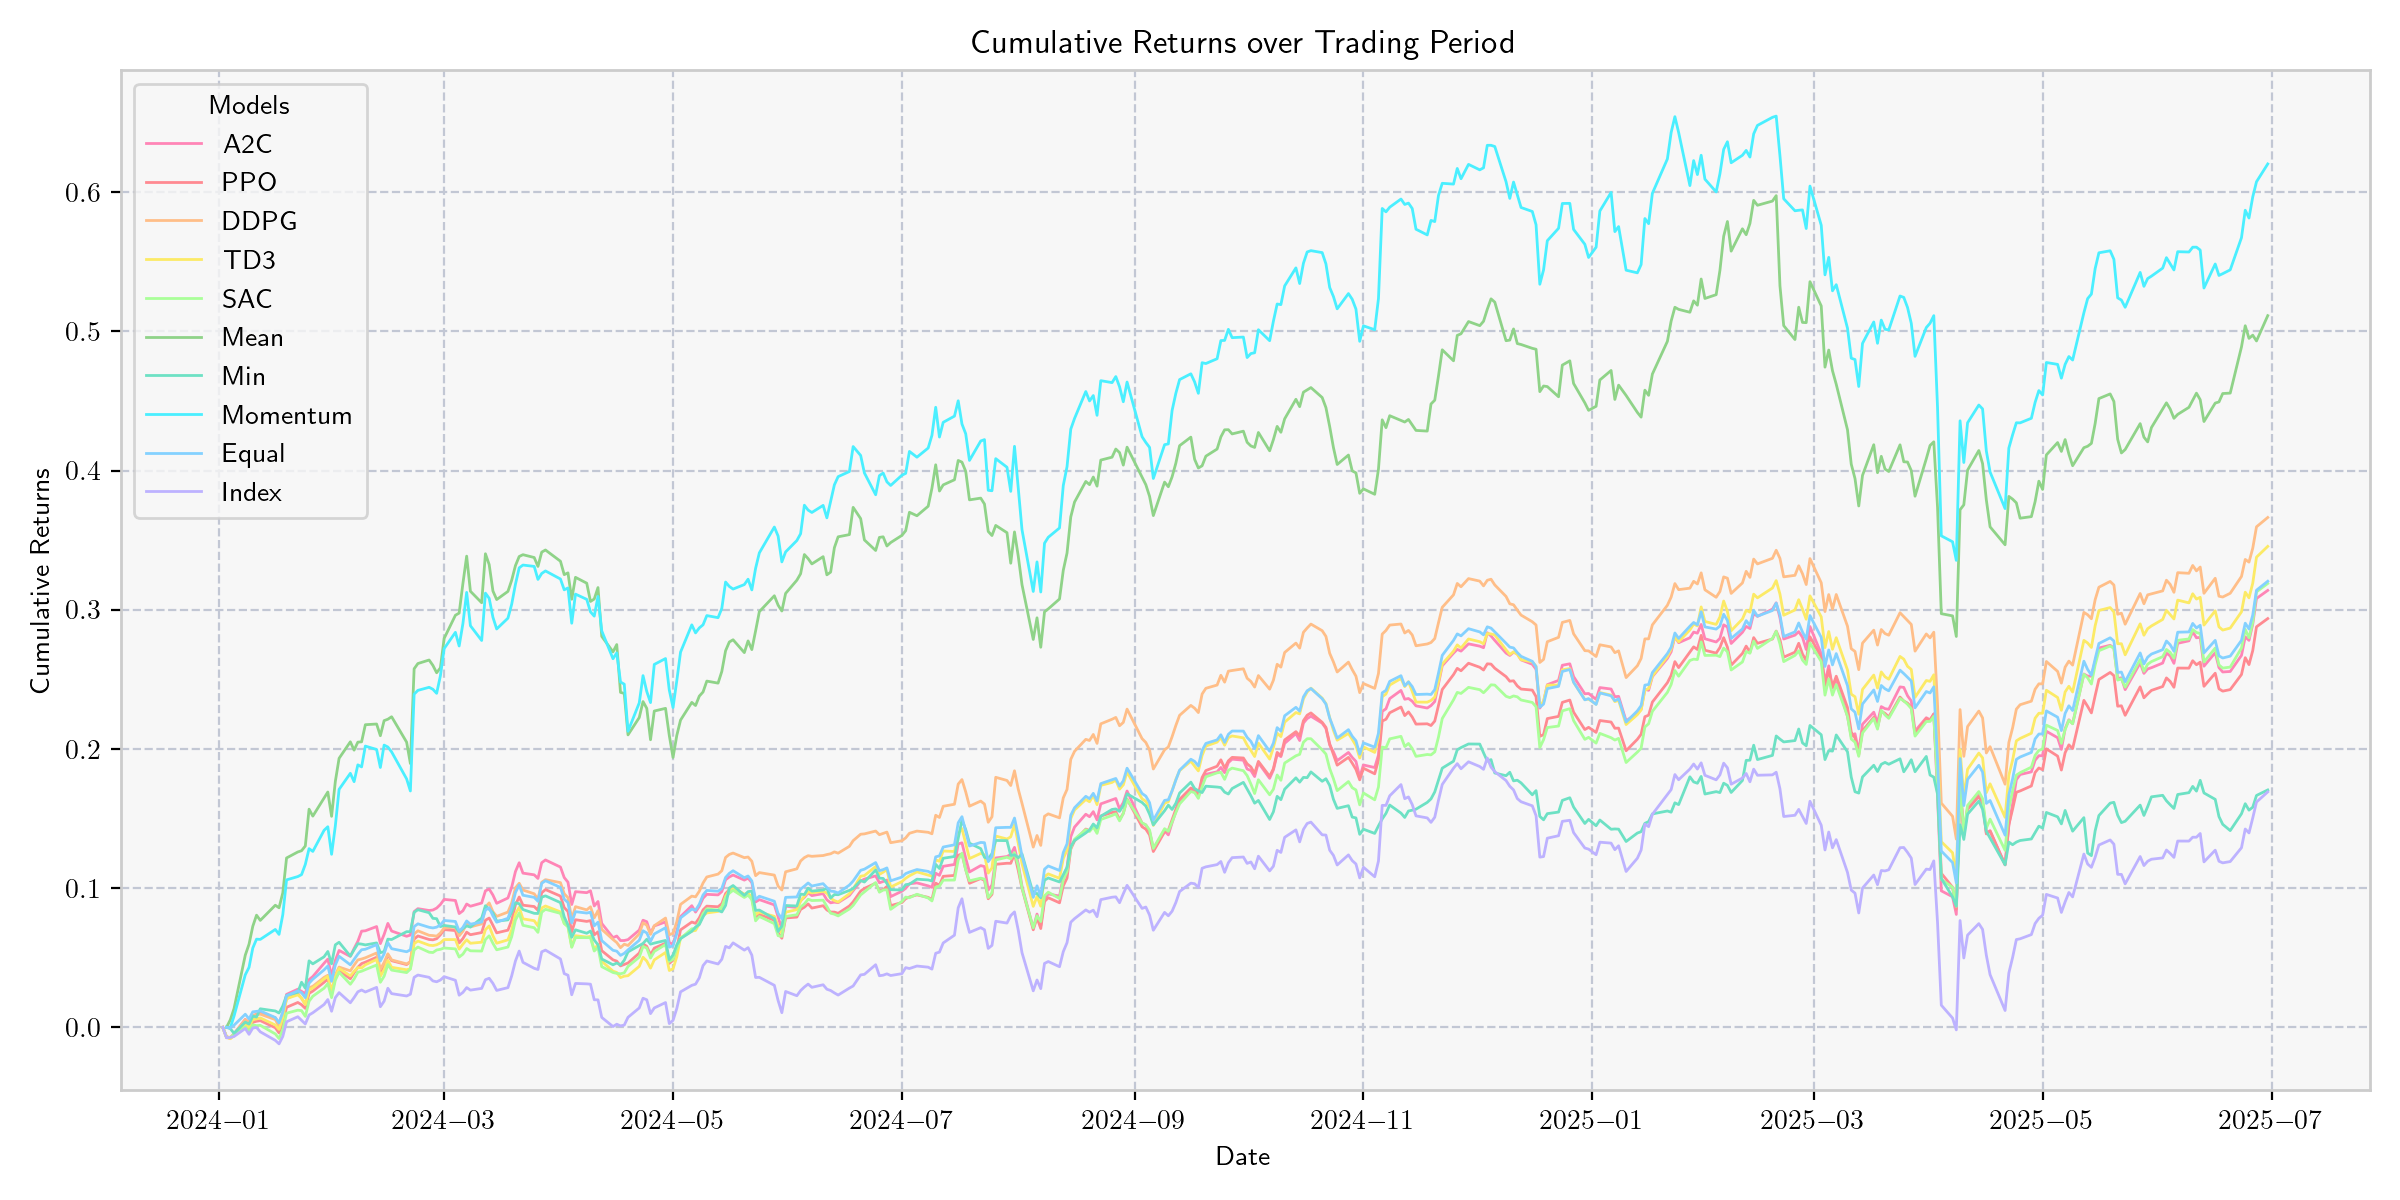
\includegraphics[width=\textwidth]{figures/dowjones30_indicators_cumulative_returns.png}
    \caption{Evolution of the Cumulative Returns for the DowJones30 dataset with the \acrshort{ohlcv} prices and indicators environment representation.}
    \label{fig:dowjones30_indicators_cumulative_returns}
\end{figure}

\begin{longtable}{|p{2cm}|p{2.1cm}|p{2.1cm}|p{2.1cm}|p{1.5cm}|p{2cm}|}
    \caption{Algorithm comparison results for the DowJones30 dataset. The colours correspond to the best performing configurations, with blue for the best performing \acrshort{drl} algorithm and green for the best benchmark.}
    \label{tab:experiment_algorithms_dow30} 
    \\ 
    \hline
    \textbf{Algorithm / Benchmark} & \textbf{Cumulative return} & \textbf{Annualised return} & \textbf{Annualised volatility} & \textbf{Sharpe ratio} & \textbf{Max drawdown}  \\ \midrule
    \endfirsthead

    \hline
    \textbf{Algorithm / Benchmark} & \textbf{Cumulative return} & \textbf{Annualised return} & \textbf{Annualised volatility} & \textbf{Sharpe ratio} & \textbf{Max drawdown}  \\ \midrule
    \endhead

    \endfoot
    \hline

    \textbf{A2C} & 0.2020 & 0.3139 & 0.1559 & 1.2575 & -0.1716 \\ \hline
    \textbf{PPO} & 0.1895 & 0.2937 & 0.1487 & 1.2407 & -0.1556 \\ \hline
    \textbf{DDPG} & \textcolor{blue}{0.2341} & 0.3663 & 0.1486 & \textcolor{blue}{1.4896} & -0.1546 \\ \hline
    \textbf{TD3} & 0.2214 & 0.3456 & 0.1517 & 1.3938 & -0.1609 \\ \hline
    \textbf{SAC} & 0.2050 & 0.3189 & 0.1480 & 1.3340 & -0.1538 \\ \midrule
    \textbf{Mean} & 0.3218 & 0.5114 & 0.1839 & 1.6096 & -0.1983 \\ \hline
    \textbf{Min} & 0.1123 & 0.1705 & 0.1157 & 0.9777 & -0.1066 \\ \hline
    \textbf{Momentum} & \textcolor{green}{0.3855} & 0.6204 & 0.1990 & \textcolor{green}{1.7388} & -0.1929 \\ \hline
    \textbf{Equal} & 0.2066 & 0.3205 & 0.1476 & 1.3461 & -0.1541 \\ \hline
    \textbf{Index} & 0.1110 & 0.1692 & 0.1532 & 0.7635 & -0.1637 \\ \hline
\end{longtable}

The results show that all the algorithms outperform the index for all the considered metrics, as well as the min-variance portfolio. Out of all the \acrshort{drl} algorithms, \acrshort{ddpg} achieves the highest cumulative return of 23.41\% and a Sharpe ratio of 1.49, followed by \acrshort{td3} with a cumulative return of 22.14\% and a Sharpe ratio of 1.39, while \acrshort{ppo} has the worst performance of the five with a cumulative return of 18.95\% and a Sharpe ratio of 1.24. However, none of these outperform the mean-variance and momentum benchmark strategies, with the latter achieving a Sharpe ratio of 1.74 and a cumulative return of 38.55\%, which is significantly higher than the performance of the \acrshort{drl} algorithms. 

%% ALL IN ALL GENERIC RESULTS

\subsection{Environment Representation} \label{sec:environment-representation}

Another source of variability in the performance of the algorithms is the environment representation. In this section, the results of comparing the \acrshort{drl} algorithms on different environment representations are presented. For the experiment to be meaningful, it has been performed on the DowJones30, the currencies and the commodities datasets. This choice provides the ability to compare the performance of the algorithms across different asset classes, while also allowing for a more manageable computational cost. The table \ref{tab:experiment_environment_sharpe} compares the performance according to the Sharpe ratio and, in Appendix \ref{app:experiment_environment_representation}, according to the cumulative return.

\begin{longtable}{|p{2cm}|p{2.2cm}|p{2cm}|p{2cm}|p{2.2cm}|p{2cm}|}
    \hline
    \textbf{Algorithm} & \textbf{Dataset} & \textbf{Simple} & \textbf{Indicators} & \textbf{Covariance} & \textbf{Complete} \\ \midrule
    \endfirsthead

    \hline
    \textbf{Algorithm} & \textbf{Dataset} & \textbf{Simple} & \textbf{Indicators} & \textbf{Covariance} & \textbf{Complete}  \\ \midrule
    \endhead

    \caption{Environment representation experiment comparison according to the Sharpe ratio.}
    \label{tab:experiment_environment_sharpe}

    \endfoot

    \hline  
    \multirow{3}{*}{\textbf{A2C}}
    & DowJones30 & 1.3203 & 1.2575 & 1.3615 & \textcolor{blue}{1.3929} \\ \cline{2-6}
    & Commodities & 1.1373 & \textcolor{green}{1.2881} & 1.0273 & 1.2079 \\ \cline{2-6}
    & Currencies & -0.0018 & -0.0571 & -0.0674 & -0.0053 \\ \midrule

    \multirow{3}{*}{\textbf{PPO}}
    & DowJones30 & 1.3410 & 1.2407 & \textcolor{blue}{1.3524} & 1.1890 \\ \cline{2-6}
    & Commodities & \textcolor{green}{1.2600} & 1.1256 & 1.1559 & 1.2015 \\ \cline{2-6}
    & Currencies & 0.0014 & 0.0699 & 0.0652 & 0.1399 \\ \midrule

    \multirow{3}{*}{\textbf{DDPG}}
    & DowJones30 & 1.3826 & \textcolor{blue}{1.4896} & 1.3562 & 1.3261 \\ \cline{2-6}
    & Commodities & \textcolor{green}{1.1745} & 0.9871 & 1.0731 & 1.1612 \\ \cline{2-6}
    & Currencies & 0.0528 & 0.0689 & 0.0200 & 0.0115 \\ \midrule

    \multirow{3}{*}{\textbf{TD3}}
    & DowJones30 & \textcolor{blue}{1.4911} & 1.3938 & 1.1792 & 1.2084 \\ \cline{2-6}
    & Commodities & \textcolor{green}{1.4537} & 0.9776 & 1.0462 & 1.2388 \\ \cline{2-6}
    & Currencies & 0.0807 & -0.0088 & -0.0086 & -0.0436 \\ \midrule
    \pagebreak

    \multirow{3}{*}{\textbf{SAC}}
    & DowJones30 & 0.9769 & 1.3340 & \textcolor{blue}{1.4670} & 1.3017 \\ \cline{2-6}
    & Commodities & \textcolor{green}{1.3727} & 1.1973 & 1.1773 & 1.0500 \\ \cline{2-6}
    & Currencies & 0.0806 & 0.1771 & -0.1441 & 0.2550 \\ \midrule

\end{longtable}

The results show that the performance of the algorithms varies significantly across different environment representations. For the DowJones30 dataset, the \acrshort{ohlcv} prices representation achieves the highest Sharpe ratio of 1.49 for \acrshort{td3}, closely followed by the \acrshort{ohlcv} prices with indicators. The \acrshort{ohlcv} prices with covariance representation achieves 1.47 for \acrshort{sac}. For the complete feature set, only the \acrshort{a2c} algorithm achieves a higher Sharpe ratio of 1.39 than the other algorithms.

For the commodities dataset, the results are completely different to those of the DowJones30. The only coincidence is that \acrshort{td3} achieves the highest Sharpe ratio and highest cumulative return in the simple feature set. Moreover, when looking at this dataset, explicitly adding the covariance to the environment representation does not lead to better performance in terms of Sharpe ratio.

Finally, for the currencies dataset, the performance of the algorithms is significantly lower, going negative in some cases. A possible reason is the particular set of hyper-parameters used. 

\subsection{Hyper-parameter Tuning} \label{sec:hyper-parameter-tuning}

As has been mentioned in the above experiments, the performance of the algorithms is substantially influenced by the choice of hyper-parameters. Ideally, a systematic approach should be employed to find the optimal hyper-parameters for each algorithm, dataset and environment representation combination. However, due to the computational cost of hyper-parameter tuning, it was only performed for the DowJones30 dataset with the \acrshort{ohlcv} and indicators environment representations over five trials. The results for each of the algorithms with the default hyper-parameters versus the tuned hyper-parameters are presented in Table \ref{tab:experiment_hyperparameters_dow30} for the two features sets: simple and with indicators.

\begin{longtable}{|c|c|c|c|c|c|}
    \caption{Hyper-parameter tuning experiment results for the DowJones30 dataset for simple and indicators feature set. The colours correspond to the best performing configurations, with blue for the best performance on the simple feature set and green for the indicators one.}
    \label{tab:experiment_hyperparameters_dow30}
    \\ 
    \hline
    \multirow{2}{*}{\textbf{Algorithm}} & \multirow{2}{*}{\textbf{Metric}} & \multicolumn{2}{c|}{\textbf{Simple}} & \multicolumn{2}{c|}{\textbf{Indicators}} \\
\cline{3-6}
     &  & \textbf{Default} & \textbf{Tuned} & \textbf{Default} & \textbf{Tuned} \\ \midrule
    \endfirsthead

    \hline
    \multirow{2}{*}{\textbf{Algorithm}} & \multirow{2}{*}{\textbf{Metric}} & \multicolumn{2}{c|}{\textbf{Simple}} & \multicolumn{2}{c|}{\textbf{Indicators}} \\
\cline{3-6}
     &  & \textbf{Default} & \textbf{Tuned} & \textbf{Default} & \textbf{Tuned} \\ \midrule
    \endhead

    \endfoot
 
    \multirow{2}{*}{\textbf{A2C}}
    & Cumulative Return & 0.3387 & 0.3491 & 0.3139 & 0.3573 \\ \cline{2-6}
    & Sharpe ratio & 1.3203 & \textcolor{blue}{1.4307} & 1.2575 & \textcolor{green}{1.3994} \\ \midrule

    \multirow{2}{*}{\textbf{PPO}}
    & Cumulative Return & 0.3174 & 0.2844 & 0.2937 & 0.3134 \\ \cline{2-6}
    & Sharpe ratio & \textcolor{blue}{1.3410} & 1.1939 & 1.2407 & \textcolor{green}{1.3679} \\ \midrule

    \multirow{2}{*}{\textbf{DDPG}}
    & Cumulative Return & 0.3454 & 0.27404 & 0.3663 & 0.4086 \\ \cline{2-6}
    & Sharpe ratio & \textcolor{blue}{1.3826} & 1.2088 & 1.4896 & \textcolor{green}{1.5597} \\ \midrule

    \multirow{2}{*}{\textbf{TD3}}
    & Cumulative Return & 0.3902 & 0.2974 & 0.3456 & 0.2891 \\ \cline{2-6}
    & Sharpe ratio & \textcolor{blue}{1.4911} & 1.2354 & \textcolor{green}{1.3938} & 1.2332 \\ \midrule

    \multirow{2}{*}{\textbf{SAC}}
    & Cumulative Return & 0.2243 & 0.3703 & 0.3189 & 0.2646 \\ \cline{2-6}
    & Sharpe ratio & 0.9769 & \textcolor{blue}{1.4521} & \textcolor{green}{1.3340} & 1.1688 \\ \midrule
\end{longtable}

By comparing the data presented in these tables, it is clear that finding the optimal configuration can have a significant impact on the performance of the algorithms. For instance, although the cumulative return for \acrshort{a2c} in the simple feature set only improves by 1\%, the Sharpe ratio increases from 1.32 to 1.43, meaning that the algorithm learns to better balance risk while maximising returns. Another example is the \acrshort{sac} algorithm, which achieves a better performance than that of the default configuration. However, for the \acrshort{ppo}, \acrshort{ddpg} and \acrshort{td3} algorithms, there are no improvements and the default hyper-parameters perform better. Similarly, when looking at the indicators feature set, not all the algorithms show sign of improvements. This means that, for that particular algorithm, dataset and environment representation combination, the optimal hyper-parameter configuration has not been found. Understandably, due to the limited computational resources, the hyper-parameter search was very limited to only five runs, which is not sufficient for a thorough search.

\section{Explainability Results} \label{sec:explainability-framework}

A main objective of this thesis is to be able to interpret the decisions made by the \acrshort{drl} algorithms. The following explainability framework is designed to provide insights into the decision-making process of the algorithms and present the most relevant features that influence the portfolio allocation decision in a visual and human-readable manner. As described in Section \ref{sec:post_hoc_explainability}, two approaches were employed: a surrogate model and direct explanations. 

For the purposes of visualisation, the results are shown for a sample dataset of five tickers (AAPL, CSCO, HON, MSFT, V) from the \acrshort{djia} and using only the open, close, high, and low prices as the environment representation. This choice is made because explanations are more easily visualised when the number of assets and features is small. However, the explainability framework itself is general and can be applied to any number of assets and any environment representation. In practice, to support larger portfolios and more complex feature sets, an interactive dashboard could be developed, allowing users to select the relevant assets in the portfolio for which explanations are required. Moreover, only the explanations of the \acrshort{a2c} algorithm are presented, as it serves as a representative example of the framework's capabilities.

To provide interpretations, several explainability techniques were employed. The surrogate model was implemented following the proposal by de-la-Rica-Escudero et al. (2025) \cite{de-La-Rica-Escudero2025}. Although their paper does not explicitly acknowledge the use of a surrogate model nor outline the reasons for its use, it can be inferred that using a simpler transparent algorithm as a proxy provides built-in feature importance, which is a global explainability method. However, there does not seem to be any added value when using \acrshort{lime} and \acrshort{shap} as they are both model-agnostic methods capable of providing explanations for any black-box model. Consequently, direct model explanations were applied using these two methods.

\subsection{Feature Importance Results} \label{sec:feature-importance-results}

The feature importance results from the surrogate model are shown in Figure \ref{fig:feature_importance_top_features}, where the top 20 features are ranked according to the importance measure. The ranking shows that the low price of CSCO and the close price of MSFT are the two most important features, followed by the open price of CSCO. At the bottom section of the ranking, HON and AAPL features have a lower importance.

\begin{figure}
    \centering
    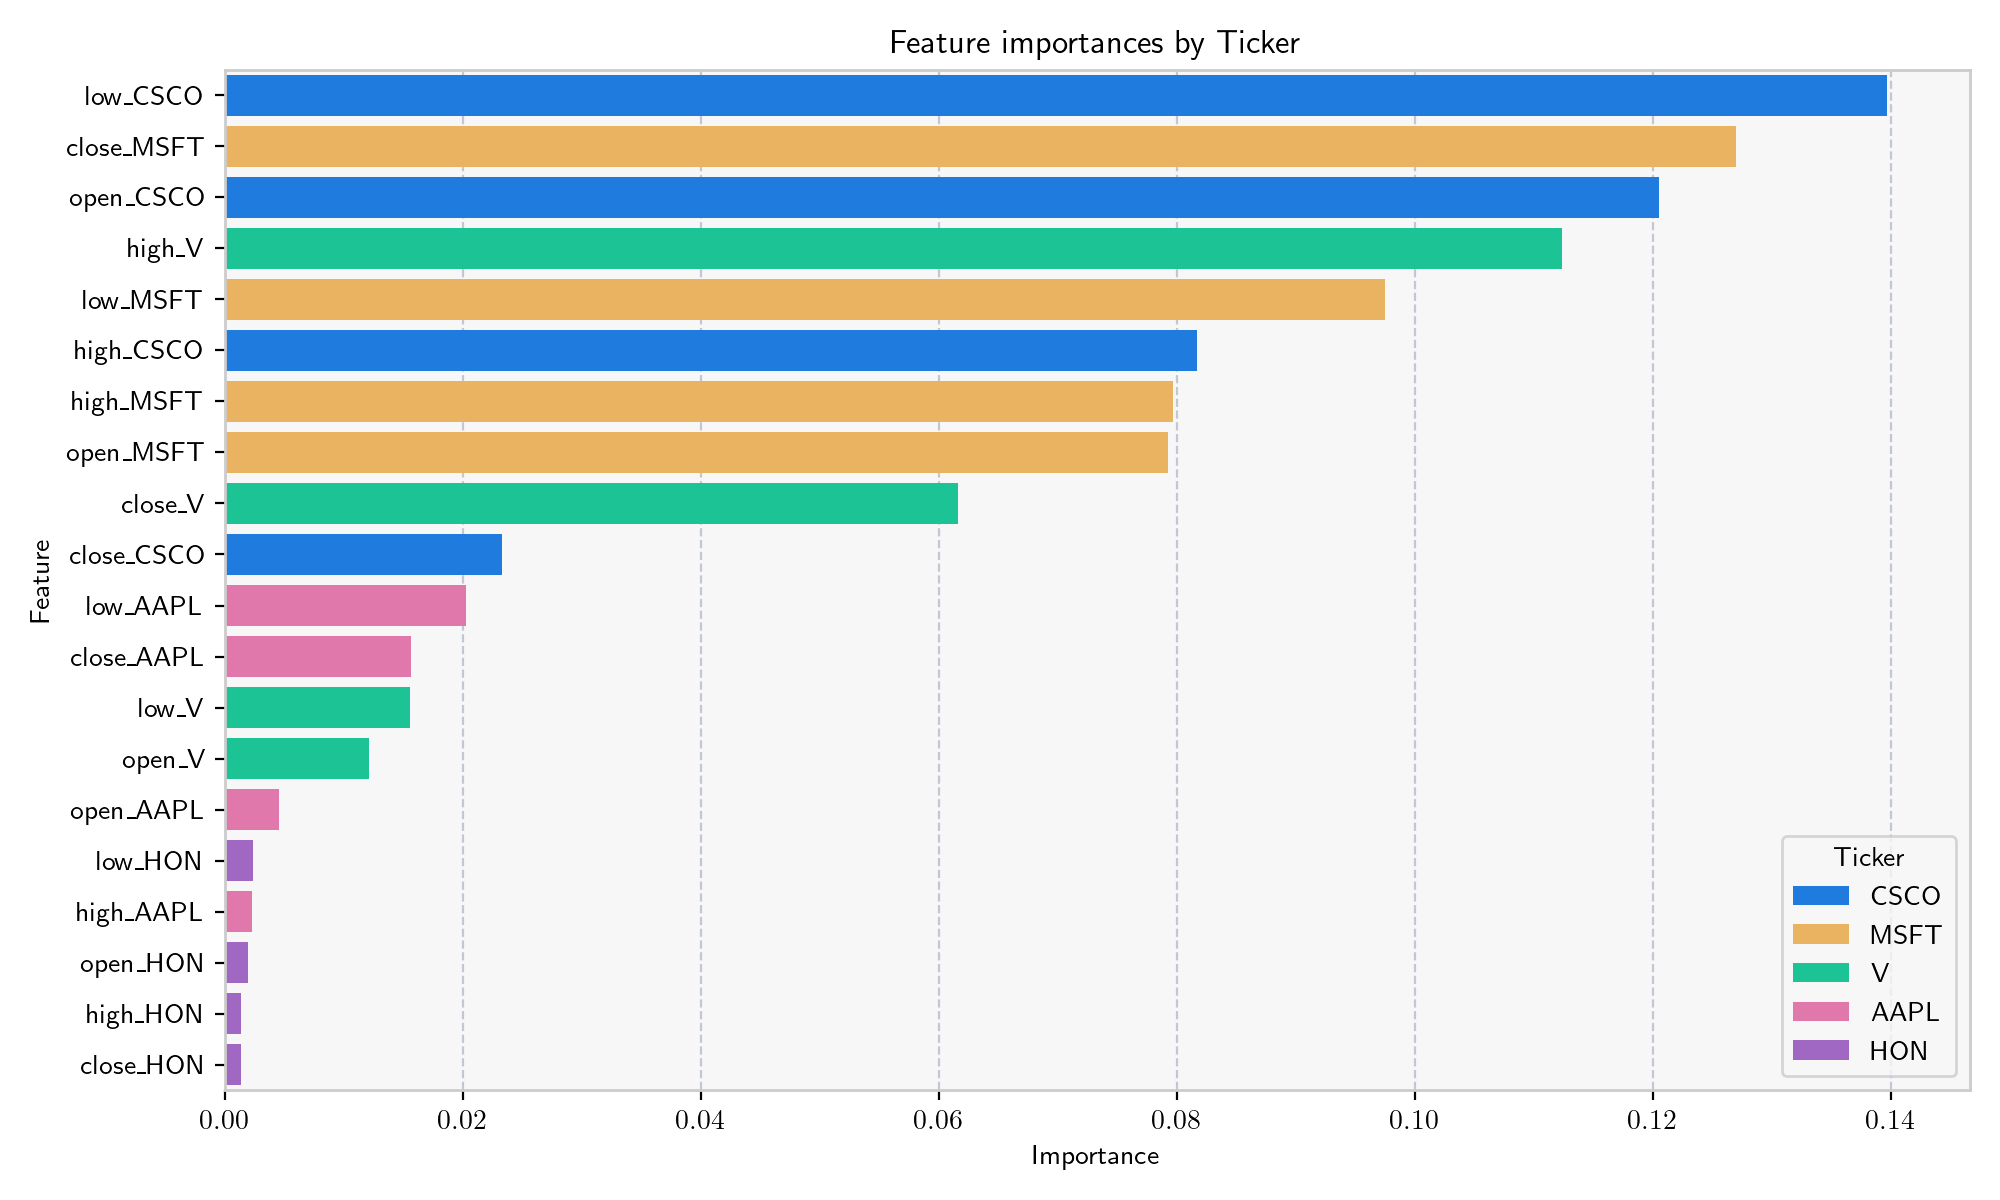
\includegraphics[width=\textwidth]{figures/feature_importance_top_features.png}
    \caption{Top features from the surrogate model according to feature importance.}
    \label{fig:feature_importance_top_features}
\end{figure}

This trend is further confirmed by looking at the mean importance of the features for each asset, as shown in Figure \ref{fig:mean_feature_importance_by_asset}. This indicates that the agent heavily relied on the performance of MSFT and CSCO to guide its portfolio allocation decisions, while the other assets played a less significant role. 

\begin{figure}
    \centering
    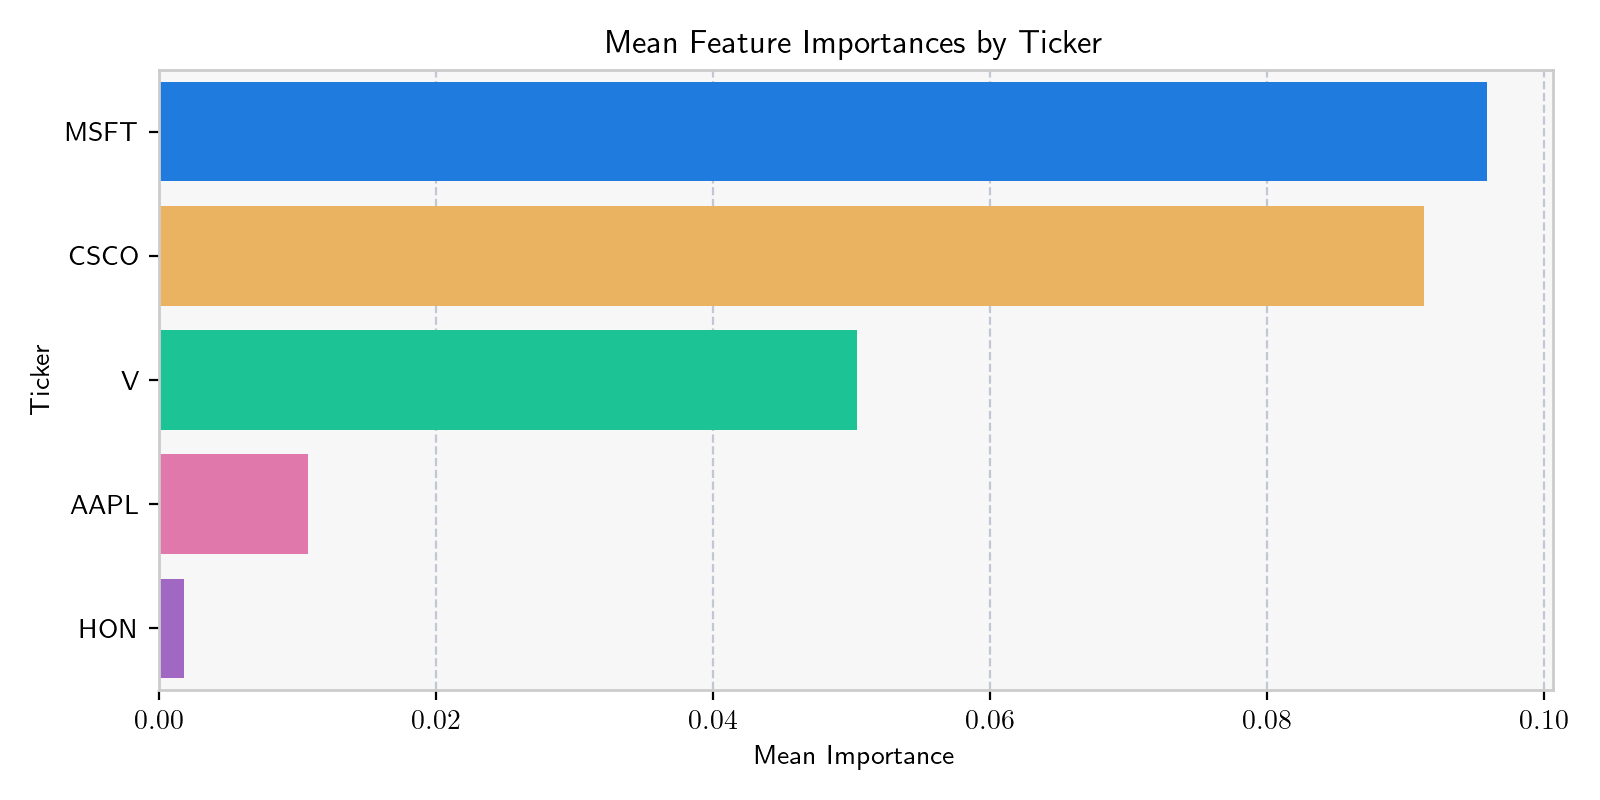
\includegraphics[width=\textwidth]{figures/feature_importance_mean_ticker.png}
    \caption{Mean feature importance per asset from the surrogate model.}
    \label{fig:mean_feature_importance_by_asset}
\end{figure}

Another interesting result about the feature importance shown in Figure \ref{fig:feature_importance_top_features} is that the different assets have a different \acrshort{ohlcv} feature importance distribution, which suggests that the agent may have developed distinct strategies for each asset. Figure \ref{fig:feature_importance_by_asset} in Appendix \ref{app:feature_importance} shows the top features grouped by asset, where it can be seen more clearly how each asset has a different most important feature. In the case of AAPL, HON and CSCO, the low price played a more critical role in informing the agent's decisions, showing how extreme price changes lead the agent to adjust the portfolio allocation. In contrast, for MSFT, the close price is the most important feature, which might imply the agent is more focused on the end of day activities of this asset. Finally, looking over all the assets, Figure \ref{fig:mean_feature_importance_by_feature} in Appendix \ref{app:feature_importance} shows how features corresponding to low and high prices contributed the most to the agent's decisions. This again indicates that the agent is sensitive to price extremes of the assets.

\subsection{Local Interpretable Model-agnostic Explanations Results} \label{sec:lime-results}

The \acrshort{lime} method provides local explanations for individual predictions, to determine the most influential features in a model's decision for a particular instance. For a particular instance, the library displays the explanation as three components:
\begin{itemize}
    \item the predicted value of the model, within a minimum and maximum range;
    \item a list of the top ten features that contributed to the model's prediction, with their corresponding values and their contribution; and
    \item a coloured list outlining the feature values, corresponding to positive (orange) or negative (blue) contribution.
\end{itemize}

Figure \ref{fig:a2c_lime_msft} presents the \acrshort{lime} explanation for the MSFT asset on a selected trading day from the test dataset, while the other assets are found in Appendix \ref{app:lime_explanations}. In this instance, the low price of V contributes positively to the MSFT allocation, while the high price of CSCO and the open price of V negatively affect the prediction by pushing it lower. Examining such local explanations across multiple time steps can help identify features that consistently impact portfolio allocation decisions.

\begin{figure}
    \centering
    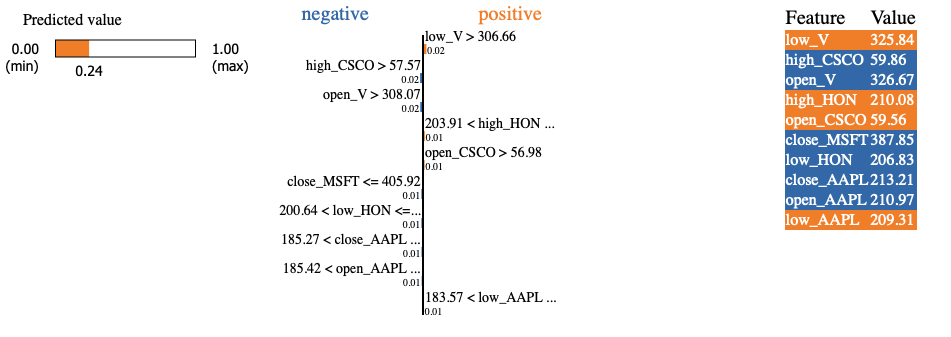
\includegraphics[width=\textwidth]{figures/a2c_lime_msft.png}
    \caption{\acrshort{lime} explanations for the \acrshort{a2c} algorithm for a specific observation in the test dataset for the MSFT asset. The orange bars indicate features that contribute positively to the prediction, while the blue bars indicate features that contribute negatively.}
    \label{fig:a2c_lime_msft}
\end{figure}

\subsection{Shapley Additive Explanations Results} \label{sec:shap-results}

The results of the \acrshort{shap} analysis provide both a global view of the feature importance across all time steps and assets, as well as a local interpretation for individual predictions. As with the case of \acrshort{lime}, instead of using a surrogate model, the explanations are extracted from the \acrshort{a2c} model directly. Since the predictions of the output are weight allocations across all portfolio assets, the \acrshort{shap} values presented in this section correspond only to AAPL, but the interpretations can be generalised to other assets and algorithms.

Figure \ref{fig:a2c_shap_beeswarm_aapl} depicts a beeswarm plot, where the x-axis represents the \acrshort{shap} value, which measures the impact of a feature on the model's output; while the y-axis displays the top features. Each point in the beeswarm plot represents a single prediction, with the point's colour indicating whether its corresponding feature value is low, coloured in blue, or high, coloured in magenta. The beeswarm plot provides a visual representation of the distribution of \acrshort{shap} values for each feature, allowing for an easy comparison of their importance. The most important feature for the AAPL asset is the low price of the MSFT asset and, by visual inspection, the high values of the low price of MSFT push the AAPL allocation lower, while the low values of the low price of MSFT push the AAPL allocation higher. However, this is not quite significant as there is a cluster of data points around the zero, indicating that, for a number of trading days, the low price of MSFT does not have an impact on AAPL's allocation. 

\begin{figure}
    \centering
    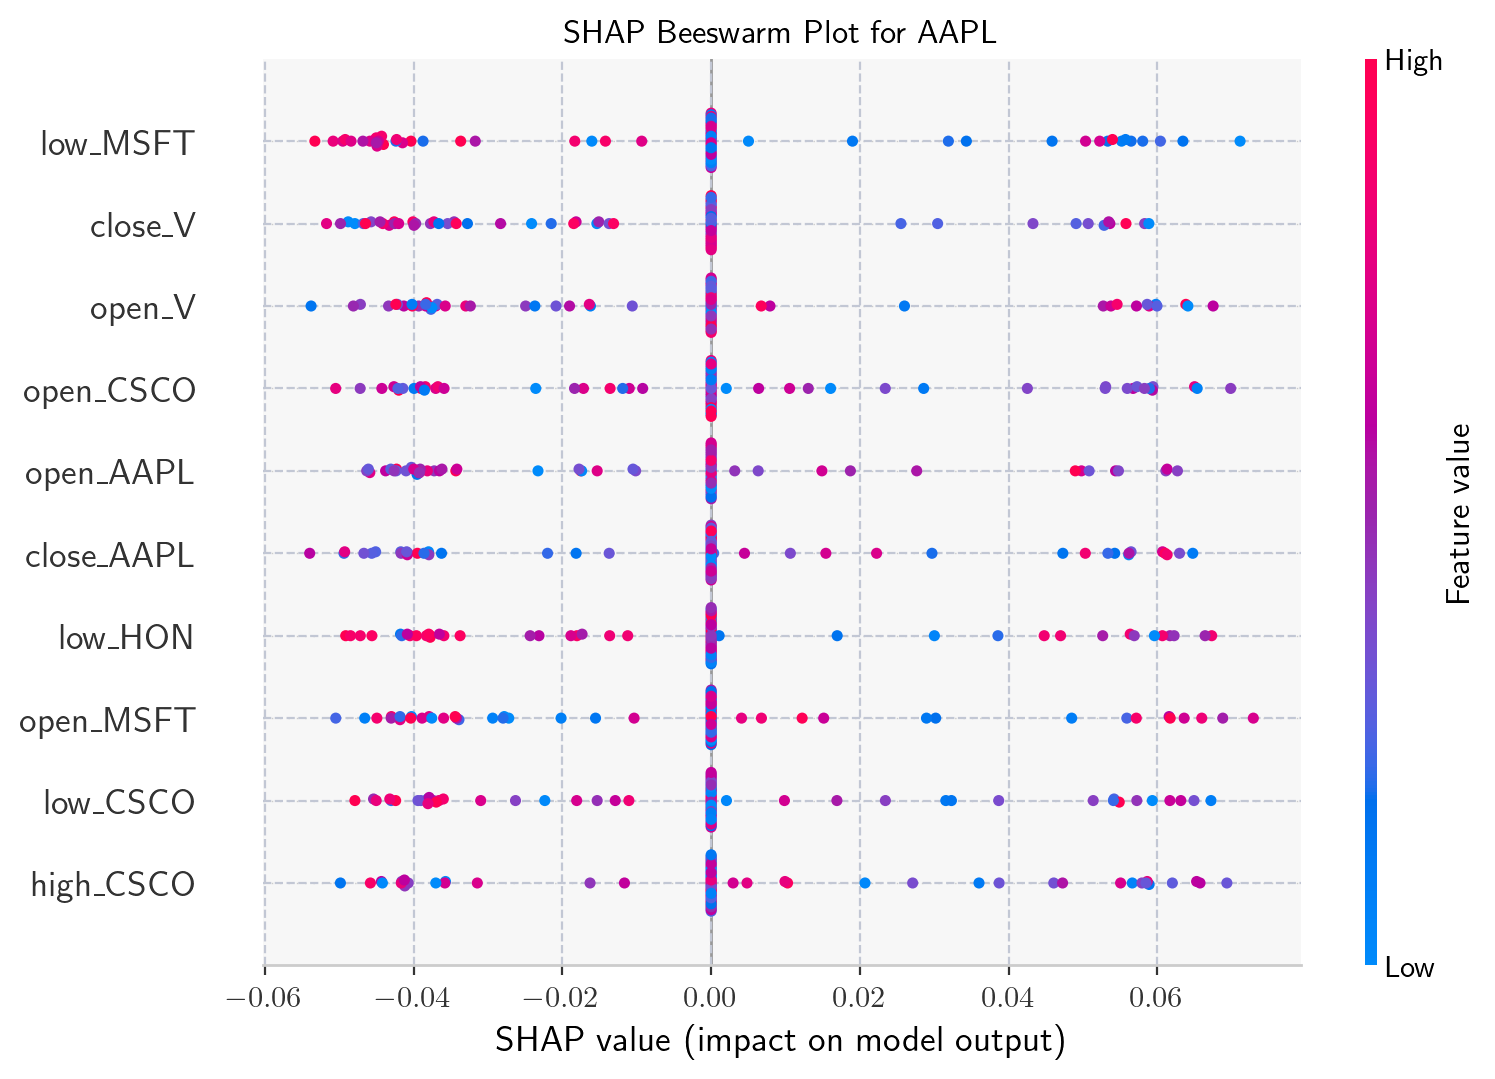
\includegraphics[width=\textwidth]{figures/a2c_shap_beeswarm_aapl.png}
    \caption{Beeswarm \acrshort{shap} explanations for the \acrshort{a2c} algorithm for the AAPL asset. The x-axis represents the \acrshort{shap} values, whilst the y-axis represents the top features. The colour indicates the feature value, with magenta being high and blue being low.}
    \label{fig:a2c_shap_beeswarm_aapl}
\end{figure}

The \texttt{shap} Python library provides numerous visualisations to explain the prediction of a model. An interesting one is the force plot, shown in Figure \ref{fig:a2c_shap_forceplot_aapl}, for the AAPL weight allocation and the contribution of all features. The force plot visualises the impact of each feature on the model's weight allocation over the entire test dataset ordered by time. Positive values, visualised in magenta, show feature contributions that push the allocation higher, while negative values, in blue, push it lower. The baseline is the average weight allocation across all time steps. 

\begin{figure}
    \centering
    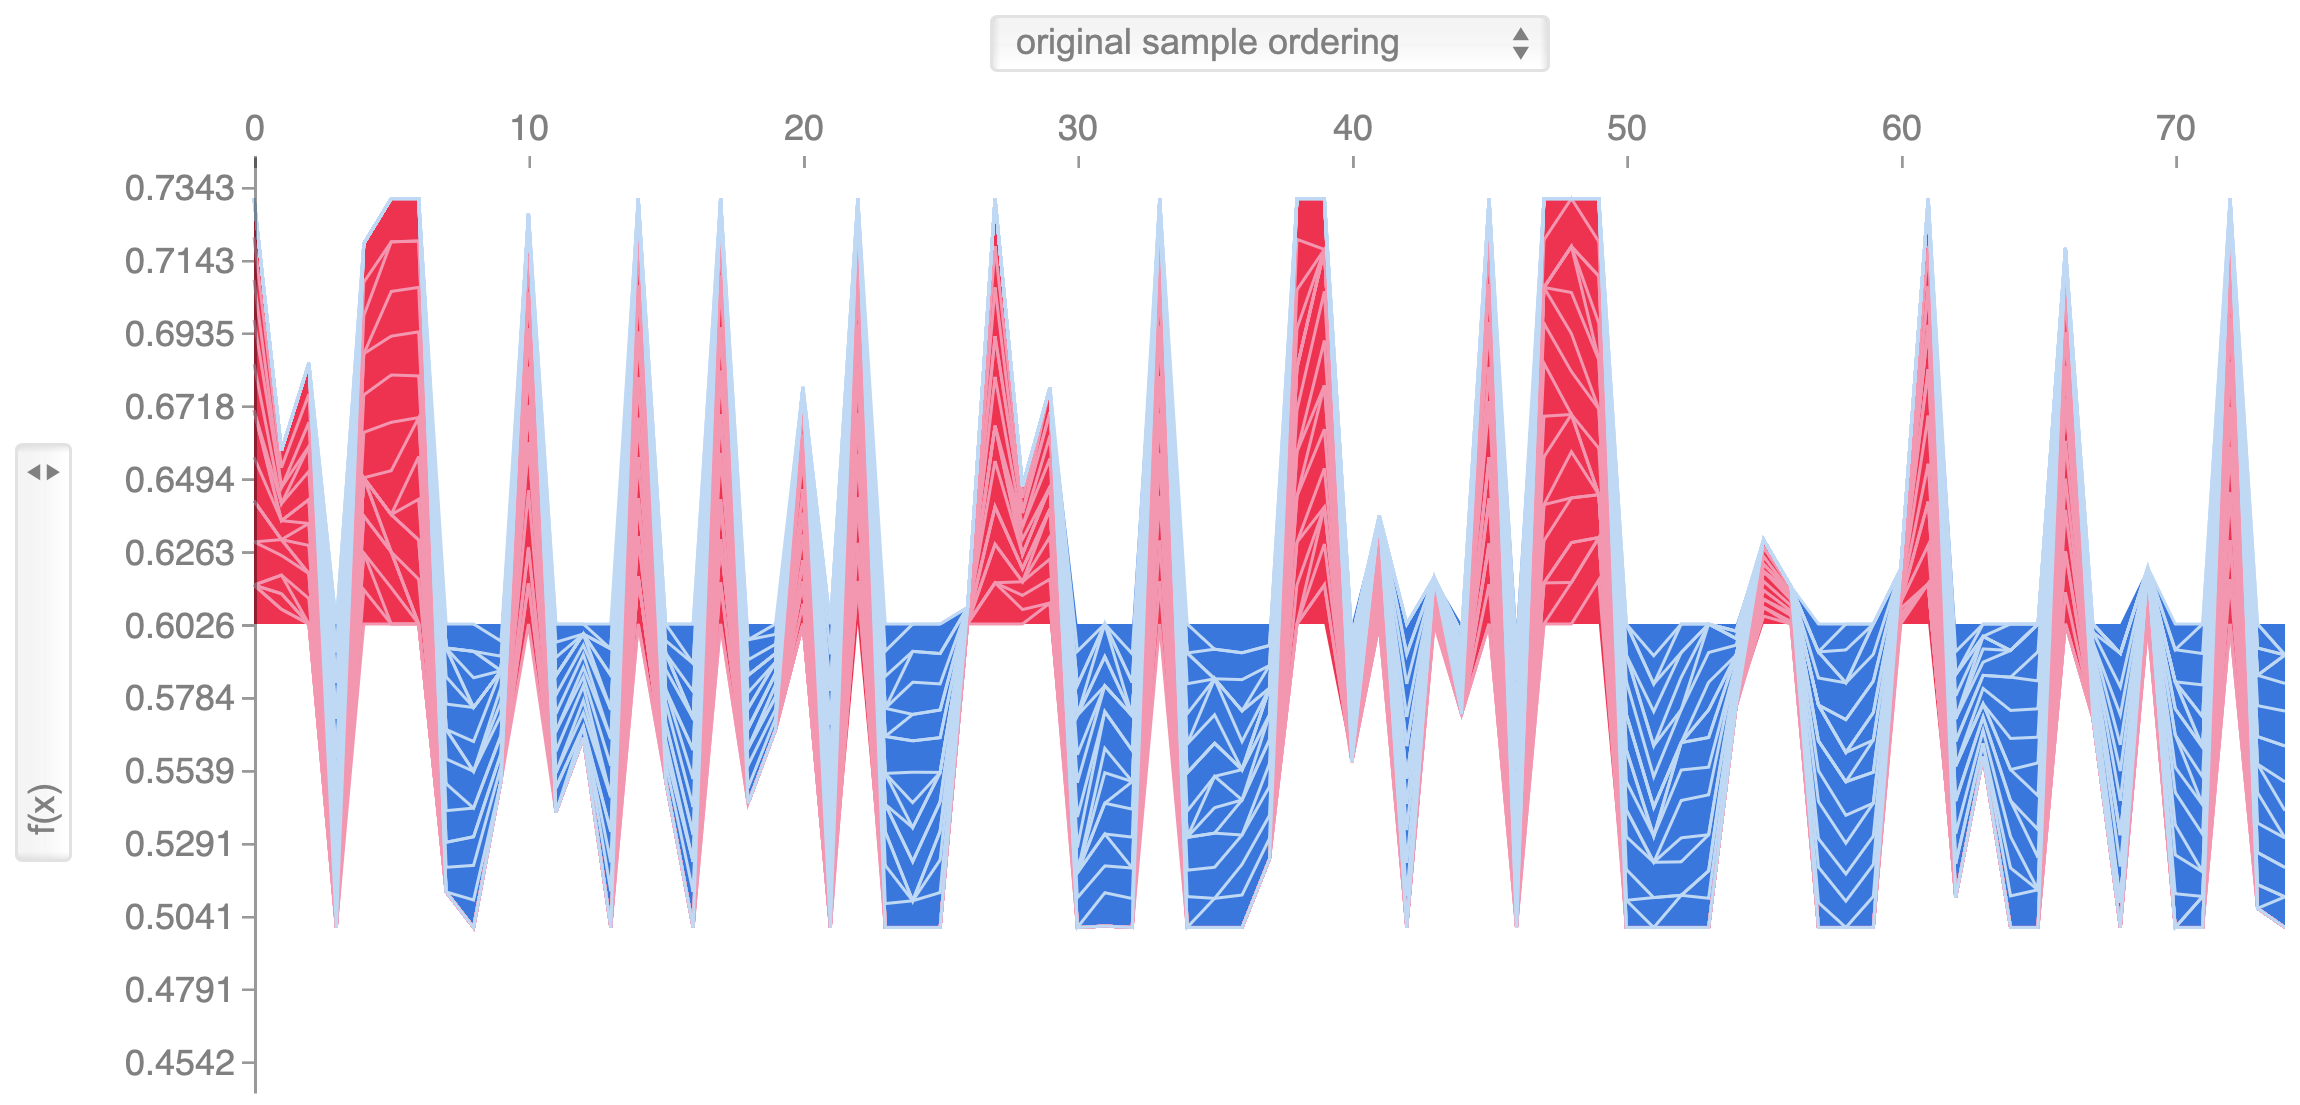
\includegraphics[width=\textwidth]{figures/a2c_shap_forceplot_aapl.png}
    \caption{\acrshort{shap} force plot for the weight allocation of the AAPL asset for the \acrshort{a2c} algorithm.}
    \label{fig:a2c_shap_forceplot_aapl}
\end{figure}

The library provides the output in \acrfull{html} format that allows interaction with the visualisation and to gain deeper insights into the model's behaviour. Using the force plot, it is possible to single out the effects of AAPL's most important feature over the test period, as shown in Figure \ref{fig:a2c_shap_forceplot_aapl_lowmsft}. Its impact is very well-defined. For approximately the first 30 time steps, it has a positive contribution, increasing AAPL's allocation, while for the remainder of the test period, it has mostly a negative contribution, decreasing the asset weight.

\begin{figure}
    \centering
    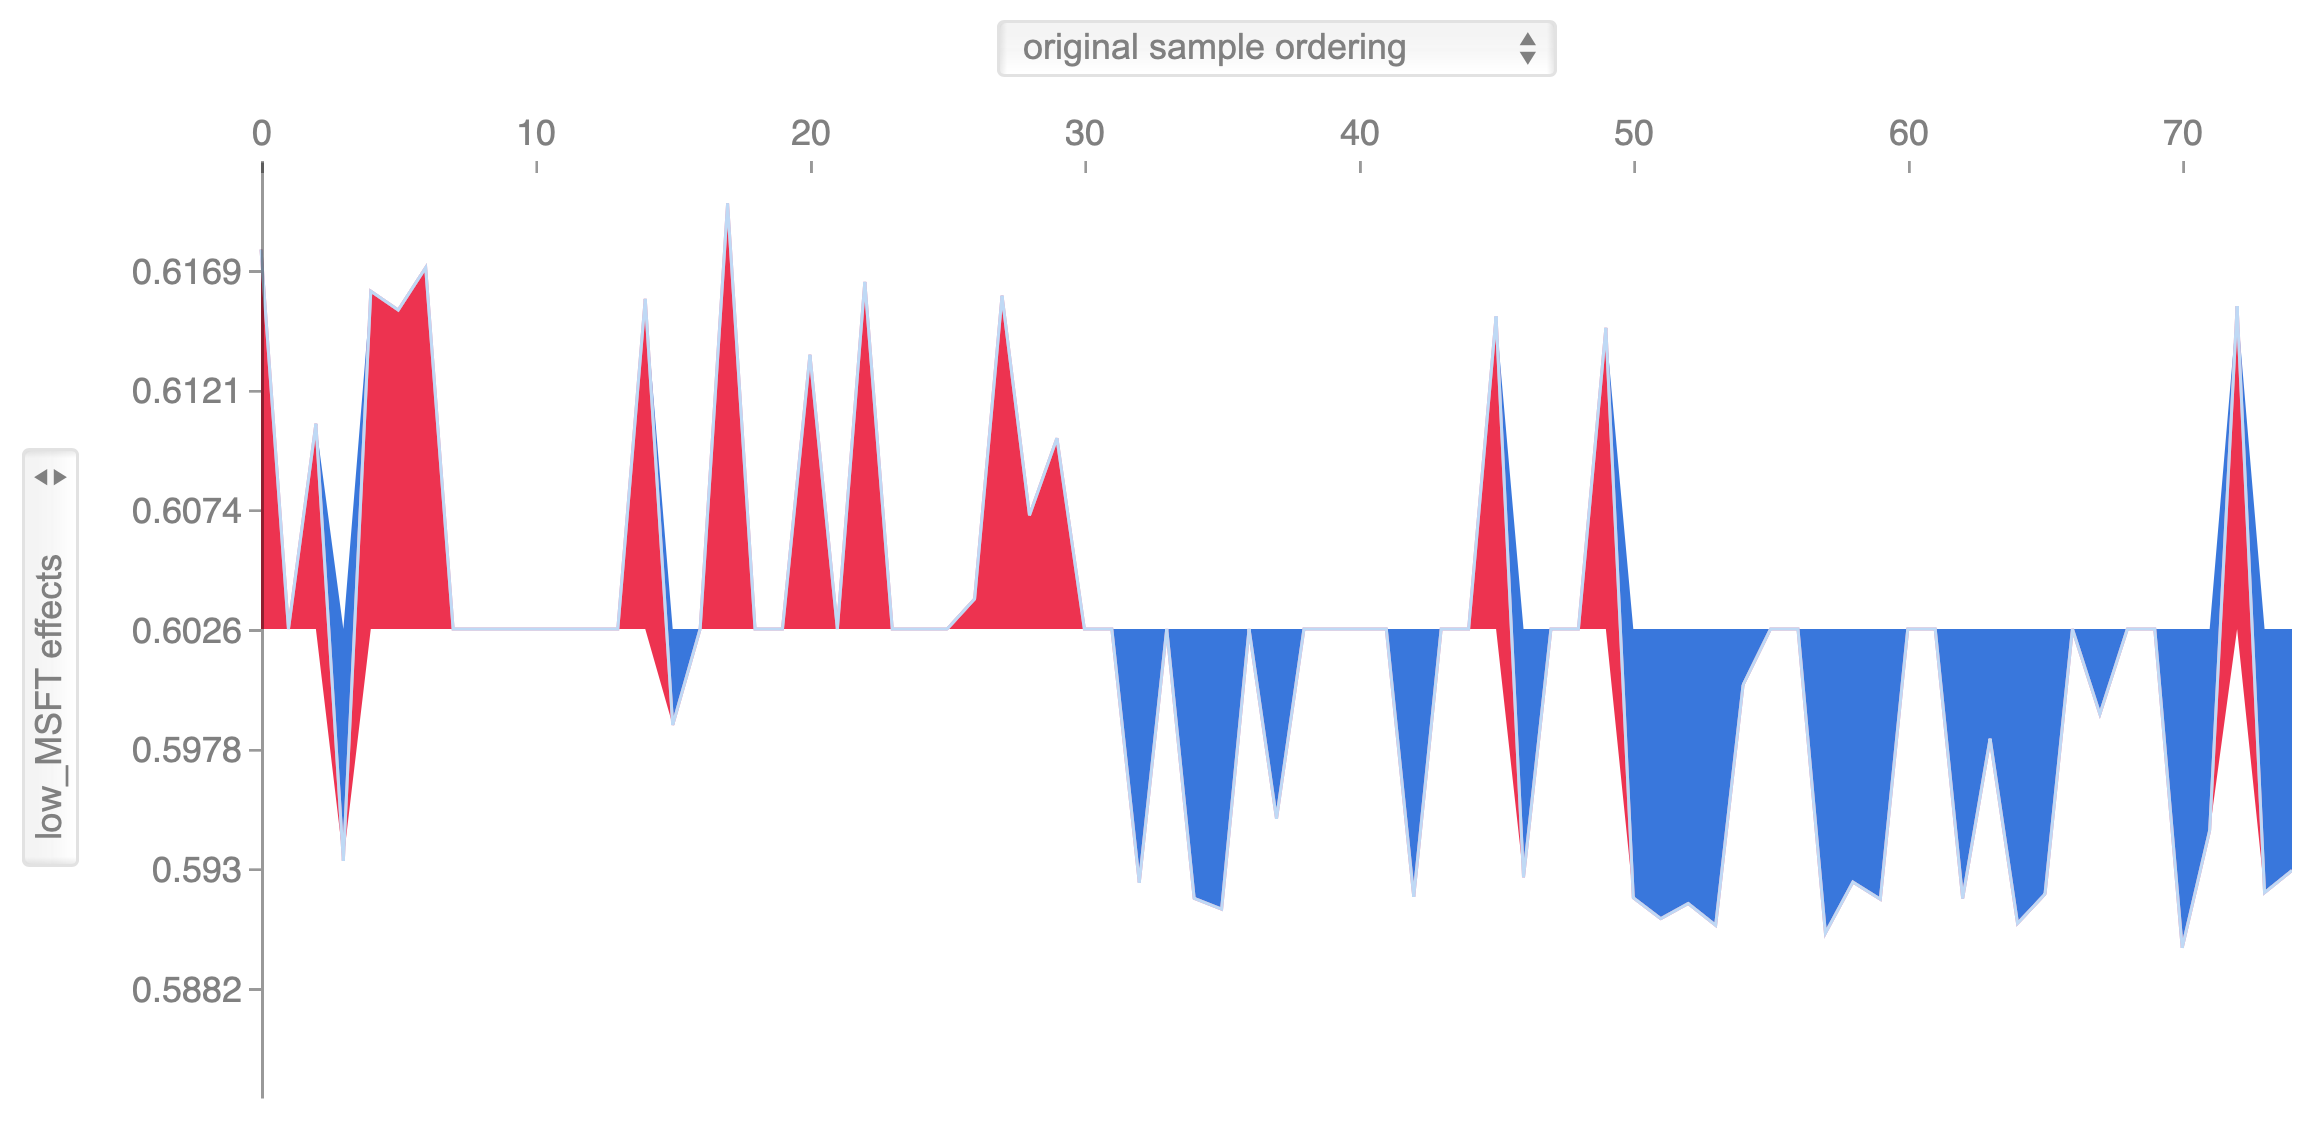
\includegraphics[width=\textwidth]{figures/a2c_shap_forceplot_aapl_lowmsft.png}
    \caption{\acrshort{shap} force plot for the impact of MSFT low price feature in the weight allocation of the AAPL asset for the \acrshort{a2c} algorithm.}
    \label{fig:a2c_shap_forceplot_aapl_lowmsft}
\end{figure}

Lundberg and Lee (2017) \cite{Lundberg2017} showed that \acrshort{lime} is a subset of \acrshort{shap} and, as a consequence, it is possible to obtain local explanations using the \texttt{shap} library. Figure \ref{fig:a2c_shap_forceplot_singleobs_aapl} shows the local explanation for the AAPL asset at a single observation of the test dataset. Although the visualisation is different, the information it provides is similar to that of \acrshort{lime}. Shown horizontally, the features in magenta push the allocation higher, while those in blue push it lower. In this case, the most important features that contribute to the allocation weight of AAPL are only features that increase the allocation and, as such, no blue features are present.

\begin{figure}
    \centering
    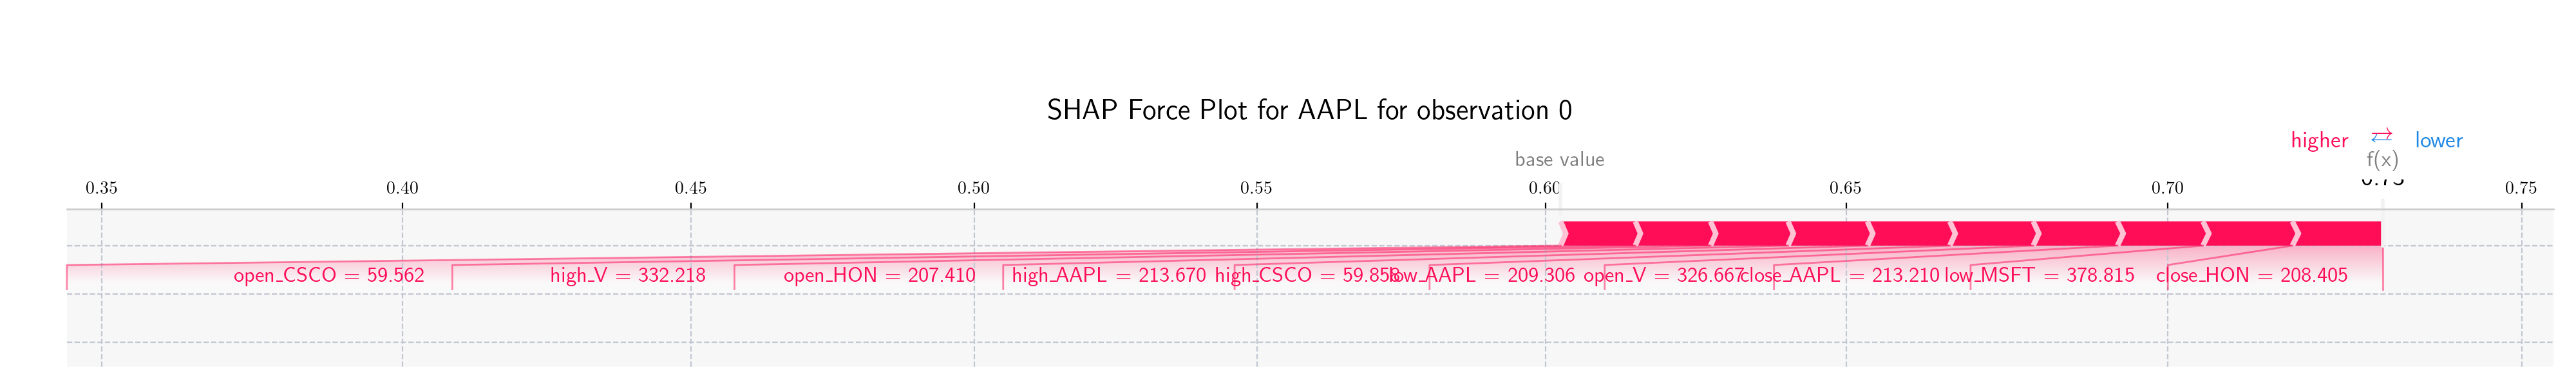
\includegraphics[width=\textwidth]{figures/a2c_shap_forceplot_singleobs_aapl.png}
    \caption{\acrshort{shap} force plot for the weight allocation of the AAPL asset for the \acrshort{a2c} algorithm at the first time step of the test dataset.}
    \label{fig:a2c_shap_forceplot_singleobs_aapl}
\end{figure}
\chapter{Legal, Social, Ethical and Professional Issues} \label{ch:issues}

The development and deployment of \acrfull{drl} algorithms to perform profitable portfolio allocation raises several legal, social, ethical and professional issues that must be considered. The incorporation of post-hoc explainable techniques to understand, interpret and clarify the decision-making process of these algorithms is a crucial step towards addressing these concerns. This chapter explores them in detail, referencing relevant regulatory frameworks and professional codes of conducts, and highlights potential mitigation strategies.

\section{Legal Issues} \label{sec:legal-issues}

When deploying \acrfull{ml} algorithms in finance, the \acrfull{eu}'s \acrfull{aiact} \cite{AIAct2024} classifies them as high-risk under Article 6 \footnote{https://artificialintelligenceact.eu/article/6/} due to their potential impact on an individuals' economic well-being. Consequently, high-risk systems must comply with Section 2, Articles 9-15 \footnote{https://artificialintelligenceact.eu/section/3-2/}, which include the obligations for risk management, data governance, documentation, transparency and human supervision. In particular, Article 13 \footnote{https://artificialintelligenceact.eu/article/13/} requires that high-risk AI systems "enable deployers to interpret a system's output". The use of explainability techniques ensures that the decision-making process of the algorithm can be understood and justified, thus adhering to the legal requirements set forth by the \acrshort{aiact}.

In addition, \Gls{algorithmictrading} systems must adhere to the \acrlong{eu} directive on \acrfull{mifid} \cite{MiFIDII} and the \acrlong{uk} \acrfull{fca} guidance on \textit{Algorithmic Trading Compliance in Wholesale Markets}. These regulations require robust governance and oversight frameworks, risk controls and thorough testing infrastructure. In this project, back-testing has been carried out to assess the algorithm's performance under varying market conditions followed by explainability techniques to enable auditability of the system.

\section{Social Issues} \label{sec:social-issues}

Despite the growing exposure to \acrfull{ai} systems with the rise of \acrfull{llm}, there is still a significant lack of understanding and trust in these systems. Some of the reasons behind this mistrust include:
\begin{itemize}
    \item The “black box” nature of models, making outputs hard to interpret.
    \item Lack of human-like qualities in the models.
    \item Perceived limitations to adapt to new situations and learn from previous mistakes.
\end{itemize}

In the context of this work, the integration of explainability techniques addresses the black box behaviour of the implemented technology by offering clear, data-driven justifications. However, transparency must also be accessible. It is essential to provide a user-friendly interface to easily access the explanations and generate plain language descriptions of those.

\section{Ethical Issues} \label{sec:ethical-issues}

The ethical implications of \acrshort{drl} in portfolio optimisation are multifaceted. The primary concern is the potential for these systems to make decisions that may not align with human values or ethical standards. For instance, if the algorithm prioritises profit maximisation without considering the social or environmental impact of its investment choices, it could lead to unethical outcomes, such as supporting companies with poor labour practices or those contributing to environmental degradation. To address this concern, the following practices can be put in place:
\begin{enumerate}
    \item the end-user should have full control over the assets included in their portfolio, allowing them to exclude companies that do not meet their ethical standards; or
    \item the environment's representation can be expanded to include ethical dimensions, like social impact or environmental sustainability metrics.
\end{enumerate}

With regard to the environment representation, it was not possible to incorporate such data as it is not readily available nor in a standardised format. 

A critical point in portfolio allocation is risk management. One of the reward functions used in this research balances return maximisation with risk minimisation, ensuring that the agent learns to avoid overly risky investments.
Additionally, the inclusion of a risk-free asset enables a safe-guard mechanism. The agent can be implemented to allocate all the resources to cash when market volatility exceeds a pre-defined threshold and resume only when said volatility decreases.

Finally, potential biases in the training data or model structure could result in allocations favouring certain industries or assets classes. This thesis mitigates such biases by constructing a portfolio from diversified indices (Appendix \ref{sec:datasets-equities}) and using explainability techniques to audit the decisions for systematic biases.

\chapter{Conclusion} \label{ch:conclusion}

This thesis has explored the application of \acrfull{drl} algorithms for optimal portfolio allocation in dynamic financial markets. The primary objective was to develop an explainable model-agnostic framework capable of enhancing the understanding of any \acrshort{drl} algorithm predictions, with the goal of providing insights into the decision-making process of these complex models as well as being a tool for auditability purposes. 

Five state-of-the-art \acrshort{drl} algorithms were implemented and evaluated on a portfolio management task. To assess the behaviour of these algorithms in different market conditions, a comprehensive experimental setup was designed, involving various datasets and environment representations. The datasets ranged from equities to commodities and currencies, each presenting unique challenges and opportunities for the \acrshort{drl} algorithms. The results demonstrated that \acrshort{drl} algorithms can effectively learn and adapt to dynamic market conditions, achieving competitive performance compared to traditional portfolio management strategies. However, the challenge remains in finding the optimal hyper-parameters, uniquely suited to each algorithm and dataset combination, in order to be able to fully exploit their potential.

Regarding the explainability aspect, the framework developed in this thesis successfully enhances the interpretability, transparency and auditability of these \gls{blackbox} models. The incorporation of feature importance through a surrogate model, \acrfull{lime} analysis and \acrfull{shap} values provides an exhaustive methodology for understanding both individual predictions and the overall decision-making process of the models over a test set. However, the results highlight the superiority of the \acrshort{shap} technique, which is capable of providing global explanations and feature importance without the need for an additional layer, in conjunction with local explanations. 

\section{Future Work} \label{sec:future-work}

Despite the comprehensive and exhaustive nature of this report, there are several areas for future research that could take this work to the next level. Starting from the main limitation of this thesis, the lack of computation resources, future work should aim to fully explore the hyper-parameter space for each of the \acrshort{drl} algorithms, datasets and environment representations. Current research in price prediction has investigated the impact of a smaller feature representation by performing feature engineering techniques, such as feature selection and dimensionality reduction, to improve model performance and reduce over-fitting.

Moreover, even in the case of optimal hyper-parameter configuration, when comparing the performance of the models to that of traditional methods the results left room for improvement. Exploring alternative reward functions, such as Sharpe ratio, incorporating additional constraints, such as transactions costs, or explicitly handling periods of high volatility, could lead to more robust and effective trading strategies. Another possibility that led to reduced performance against the benchmarks was the exclusion of the risk-free asset in the portfolio. A future direction could be to include a risk-free asset in the portfolio, which would result in a more diversified portfolio and potentially less risky. In terms of real-world scenarios, portfolios tend to be composed of different asset classes. Although this thesis explored the performance of the algorithms in different classes, forthcoming research could investigate the performance of these algorithms in multi-asset class portfolios.

Finally, for the explainability aspect, within the existing framework, it still remains to create a more user-friendly interface that allows users to provide their dataset and prediction function easily and explore the explanations generated by the model interactively. Another direction could be to explore the addition of intrinsic interpretability methods directly within the \acrshort{drl} algorithms, such as attention-based mechanisms, leading to more interpretable models. 

\pagenumbering{roman}

%%%%%% Bibliography
\renewcommand{\bibname}{References}
\bibliographystyle{ieeetr}
\bibliography{bibliography} 

%%%%%% Appendices
\appendix
\appendix

\chapter{DRL Algorithms} \label{ch:drl_algorithms}

\begin{algorithm}
\label{alg:a2c}
\caption{Advantage Actor-Critic (A2C) Pseudo-code}
\begin{algorithmic}
\State \textit{// Assume global shared parameter vectors } $\theta$ \textit{ and } $\theta_v$
\State \textit{// Assume } $N$ \textit{ parallel worker environments}
\State Initialize global step counter $T = 0$
\Repeat
    \State Reset gradients: $d\theta \gets 0$ and $d\theta_v \gets 0$
    \State Initialize empty batch storage for all workers
    \For{worker $i = 1$ to $N$}
        \State $t_{\text{start}} = t$
        \State Get state $s_t^{(i)}$ from worker $i$
        \Repeat
            \State Perform $a_t^{(i)}$ according to policy $\pi(a_t^{(i)} | s_t^{(i)}; \theta)$
            \State Receive reward $r_t^{(i)}$ and new state $s_{t+1}^{(i)}$
            \State Store $(s_t^{(i)}, a_t^{(i)}, r_t^{(i)})$ in worker $i$'s trajectory
            \State $t \gets t + 1$
        \Until{terminal $s_t^{(i)}$ or $t - t_{\text{start}} == t_{\max}$}
        
        \State $R^{(i)} = 
            \begin{cases}
                0 & \text{for terminal } s_t^{(i)} \\
                V(s_t^{(i)}, \theta_v) & \text{for non-terminal } s_t^{(i)}
            \end{cases}$
        
        \For{$j \in \{t-1, \ldots, t_{\text{start}}\}$}
            \State $R^{(i)} \gets r_j^{(i)} + \gamma R^{(i)}$
            \State Accumulate gradients w.r.t. $\theta$:
            \State \quad $d\theta \gets d\theta + \nabla_{\theta} \log \pi(a_j^{(i)} | s_j^{(i)}; \theta) (R^{(i)} - V(s_j^{(i)}; \theta_v))$
            \State Accumulate gradients w.r.t. $\theta_v$:
            \State \quad $d\theta_v \gets d\theta_v + \frac{\partial (R^{(i)} - V(s_j^{(i)}; \theta_v))^2}{\partial \theta_v}$
        \EndFor
    \EndFor
    \State \textit{// Synchronous update: wait for all workers to complete}
    \State Average gradients: $d\theta \gets \frac{1}{N} d\theta$ and $d\theta_v \gets \frac{1}{N} d\theta_v$
    \State Perform synchronous update of $\theta$ using $d\theta$ and of $\theta_v$ using $d\theta_v$
    \State $T \gets T + N \times t_{\max}$
\Until{$T > T_{\max}$}
\end{algorithmic}

\end{algorithm}

\begin{algorithm}
\label{alg:ppo}
\caption{Proximal Policy Optimization (PPO) Pseudo-code}
\begin{algorithmic}
\State \textit{// Assume initial policy parameters } $\theta_0$ \textit{ and value function parameters } $\phi_0$
\State \textit{// Hyper-parameters: } $\epsilon, \gamma, \lambda, \alpha_\pi, \alpha_v, K_{\text{epochs}}, N_{\text{minibatch}}, c_1, c_2$
\State Initialize global step counter $T \gets 0$
\For{$k = 0, 1, 2, \ldots$}
    \State Collect set of trajectories $\mathcal{D}_k = \{\tau_i\}$ by running policy $\pi_k = \pi(\theta_k)$ in environment
    \State Store transitions: $\{(s_t, a_t, r_t, s_{t+1}, \text{done}_t)\}$
    
    \For{each trajectory $\tau$ in $\mathcal{D}_k$}
        \State Compute value estimates: $V_t = V_{\phi_k}(s_t)$
        \State Compute TD residuals: $\delta_t = r_t + \gamma V_{t+1} (1 - \text{done}_t) - V_t$
        \State Compute GAE advantages: $\hat{A}_t = \sum_{l=0}^{\infty} (\gamma \lambda)^l \delta_{t+l}$
        \State Compute returns: $\hat{R}_t = \hat{A}_t + V_t$
    \EndFor
    
    \For{epoch $e = 1$ to $K_{\text{epochs}}$}
        \State Shuffle dataset $\mathcal{D}_k$
        \For{each minibatch $\mathcal{B}$ in $\mathcal{D}_k$}
            \State $r_t(\theta) = \frac{\pi_\theta(a_t | s_t)}{\pi_{\theta_k}(a_t | s_t)}$
            \State $L^{\text{CLIP}}(\theta) = \frac{1}{|\mathcal{B}|} \sum_{t \in \mathcal{B}} \min\left(r_t(\theta) \hat{A}_t, \text{clip}(r_t(\theta), 1-\epsilon, 1+\epsilon) \hat{A}_t\right)$
            \State $L^{VF}(\phi) = \frac{1}{|\mathcal{B}|} \sum_{t \in \mathcal{B}} \left(V_\phi(s_t) - \hat{R}_t\right)^2$
            \State $L(\theta, \phi) = L^{\text{CLIP}}(\theta) - c_1 L^{VF}(\phi) + c_2 S[\pi_\theta]$
            \State $\theta \gets \theta + \alpha_\pi \nabla_\theta L^{\text{CLIP}}(\theta)$
            \State $\phi \gets \phi - \alpha_v \nabla_\phi L^{VF}(\phi)$
        \EndFor
    \EndFor
    
    \State Update policy: $\theta_{k+1} = \theta$
    \State Update value function: $\phi_{k+1} = \phi$
    \State $T \gets T + |\mathcal{D}_k|$
\EndFor
\end{algorithmic}

\end{algorithm}

\begin{algorithm}
\label{alg:ddpg}
\caption{Deep Deterministic Policy Gradient (DDPG) Pseudo-code}
\begin{algorithmic}
\State \textbf{Initialise:}
\State \quad Critic network $Q_{\theta^Q}(s, a)$ and actor $\mu_{\theta^\mu}(s)$ with random weights $\theta^Q$, $\theta^\mu$
\State \quad Target networks: $\theta^{Q'} \leftarrow \theta^Q$, $\theta^{\mu'} \leftarrow \theta^\mu$
\State \quad Replay buffer $\mathcal{B}$
\State \quad Hyper-parameters: discount $\gamma$, soft update rate $\tau$, batch size $N$, exploration noise process $\mathcal{N}$, learning rates $\alpha_Q, \alpha_\mu$, total episodes $M$, steps per episode $T$
\For{episode $= 1$ to $M$}
    \State Initialise random process $\mathcal{N}$ for action exploration
    \State Receive initial state $s_1$
    \For{$t = 1$ to $T$}
        \State Select action $a_t = \mu_{\theta^\mu}(s_t) + \mathcal{N}_t$
        \State Execute $a_t$, observe reward $r_t$ and next state $s_{t+1}$
        \State Store $(s_t, a_t, r_t, s_{t+1})$ in $\mathcal{B}$
        \State Sample mini-batch $\{(s_i, a_i, r_i, s_{i+1})\}_{i=1}^N$ from $\mathcal{B}$
        \State Compute target: $y_i = r_i + \gamma Q_{\theta^{Q'}}(s_{i+1}, \mu_{\theta^{\mu'}}(s_{i+1}))$
        \State Update critic by minimising: $L(\theta^Q) = \frac{1}{N}\sum_i (y_i - Q_{\theta^Q}(s_i, a_i))^2$
        \State Update actor by policy gradient:
        \State \quad $\nabla_{\theta^\mu} J \approx \frac{1}{N}\sum_i \nabla_a Q_{\theta^Q}(s_i, a)|_{a=\mu_{\theta^\mu}(s_i)} \nabla_{\theta^\mu}\mu_{\theta^\mu}(s_i)$
        \State Update target networks:
        \State \quad $\theta^{Q'} \leftarrow \tau \theta^Q + (1 - \tau)\theta^{Q'}$
        \State \quad $\theta^{\mu'} \leftarrow \tau \theta^\mu + (1 - \tau)\theta^{\mu'}$
    \EndFor
\EndFor
\end{algorithmic}
\end{algorithm}
\chapter{State Representation} \label{app:state_representation}

\section{Technical Indicators} \label{sec:technical-indicators}

The following technical indicators are used to represent the state of the financial environment. They are calculated based on the historical price data of the assets in the portfolio:

\section{Macroeconomic Indicators} \label{sec:macroeconomic-indicators}

The following macroeconomic indicators are used to represent the state of the financial environment. They provide additional context about the market conditions and are calculated based on external data sources:


\end{document}
